\documentclass[titlepage,a4paper]{article}

\usepackage{a4wide}
\usepackage[colorlinks=true,linkcolor=black,urlcolor=blue,bookmarksopen=true]{hyperref}
\usepackage{bookmark}
\usepackage{fancyhdr}
\usepackage[spanish]{babel}
\usepackage[utf8]{inputenc}
\usepackage[T1]{fontenc}
\usepackage{graphicx}
\usepackage{float}
\usepackage[margin=0.65in]{geometry}

\pagestyle{fancy} % Encabezado y pie de página
\fancyhf{}
\fancyhead[L]{TP Diseño - Coffee Shop Analysis}
\fancyhead[R]{Sistemas Distribuidos I - FIUBA}
\renewcommand{\headrulewidth}{0.4pt}
\fancyfoot[C]{\thepage}
\renewcommand{\footrulewidth}{0.4pt}

\begin{document}
\begin{titlepage} % Carátula
	\hfill
\includegraphics[width=6cm]{logofiuba.jpg}
    \centering
    \vfill
    \Huge \textbf{TP Diseño - Coffee Shop Analysis}
    \vskip2cm
    \Large [75.74] Sistemas Distribuidos I\\
    Segundo cuatrimestre de 2025 
    \vfill
    \begin{tabular}{ | l | l | l |}
      \hline
      Avecilla, Ignacio & 105067& iavecilla@fi.uba.ar\\ \hline
      Avila, Gaston& 104482& gavila@fi.uba.ar\\ \hline
      Muñoz, Juan Martín & 106699& jmmunoz@fi.uba.ar\\ \hline
  	\end{tabular}
    \vfill
    \vfill
\end{titlepage}

\tableofcontents % Índice general
\newpage

\section{Alcance}\label{sec:alcance}
\paragraph{El presente informe presenta la documentación de un sistema distribuido flexible, robusto y escalable, capaz de resolver las consultas otorgadas por la catedra con una cantidad de unidades de procesamiento mayor o igual a uno.}

\paragraph{Las consultas a resolver son:}
\begin{enumerate}
    \item Transacciones (Id y monto) realizadas durante 2024 y 2025 entre las 06:00 AM y las
11:00 PM con monto total mayor o igual a 75.
\item Productos más vendidos (nombre y cant) y productos que más ganancias han generado
(nombre y monto), para cada mes en 2024 y 2025.
\item TPV (Total Payment Value) por cada semestre en 2024 y 2025, para cada sucursal, para
transacciones realizadas entre las 06:00 AM y las 11:00 PM.
\item Fecha de cumpleaños de los 3 clientes que han hecho más compras durante 2024 y
2025, para cada sucursal.
\end{enumerate}

\section{Arquitectura}\label{sec:arquitectura}

\subsection{Vista Física}
\paragraph{Se muestra la enteridad del sistema y las conexiones existentes entre las diversas entidades del sistema.}

\subsubsection{Diagrama de Robustez}
\begin{figure}[H]
	\centering
	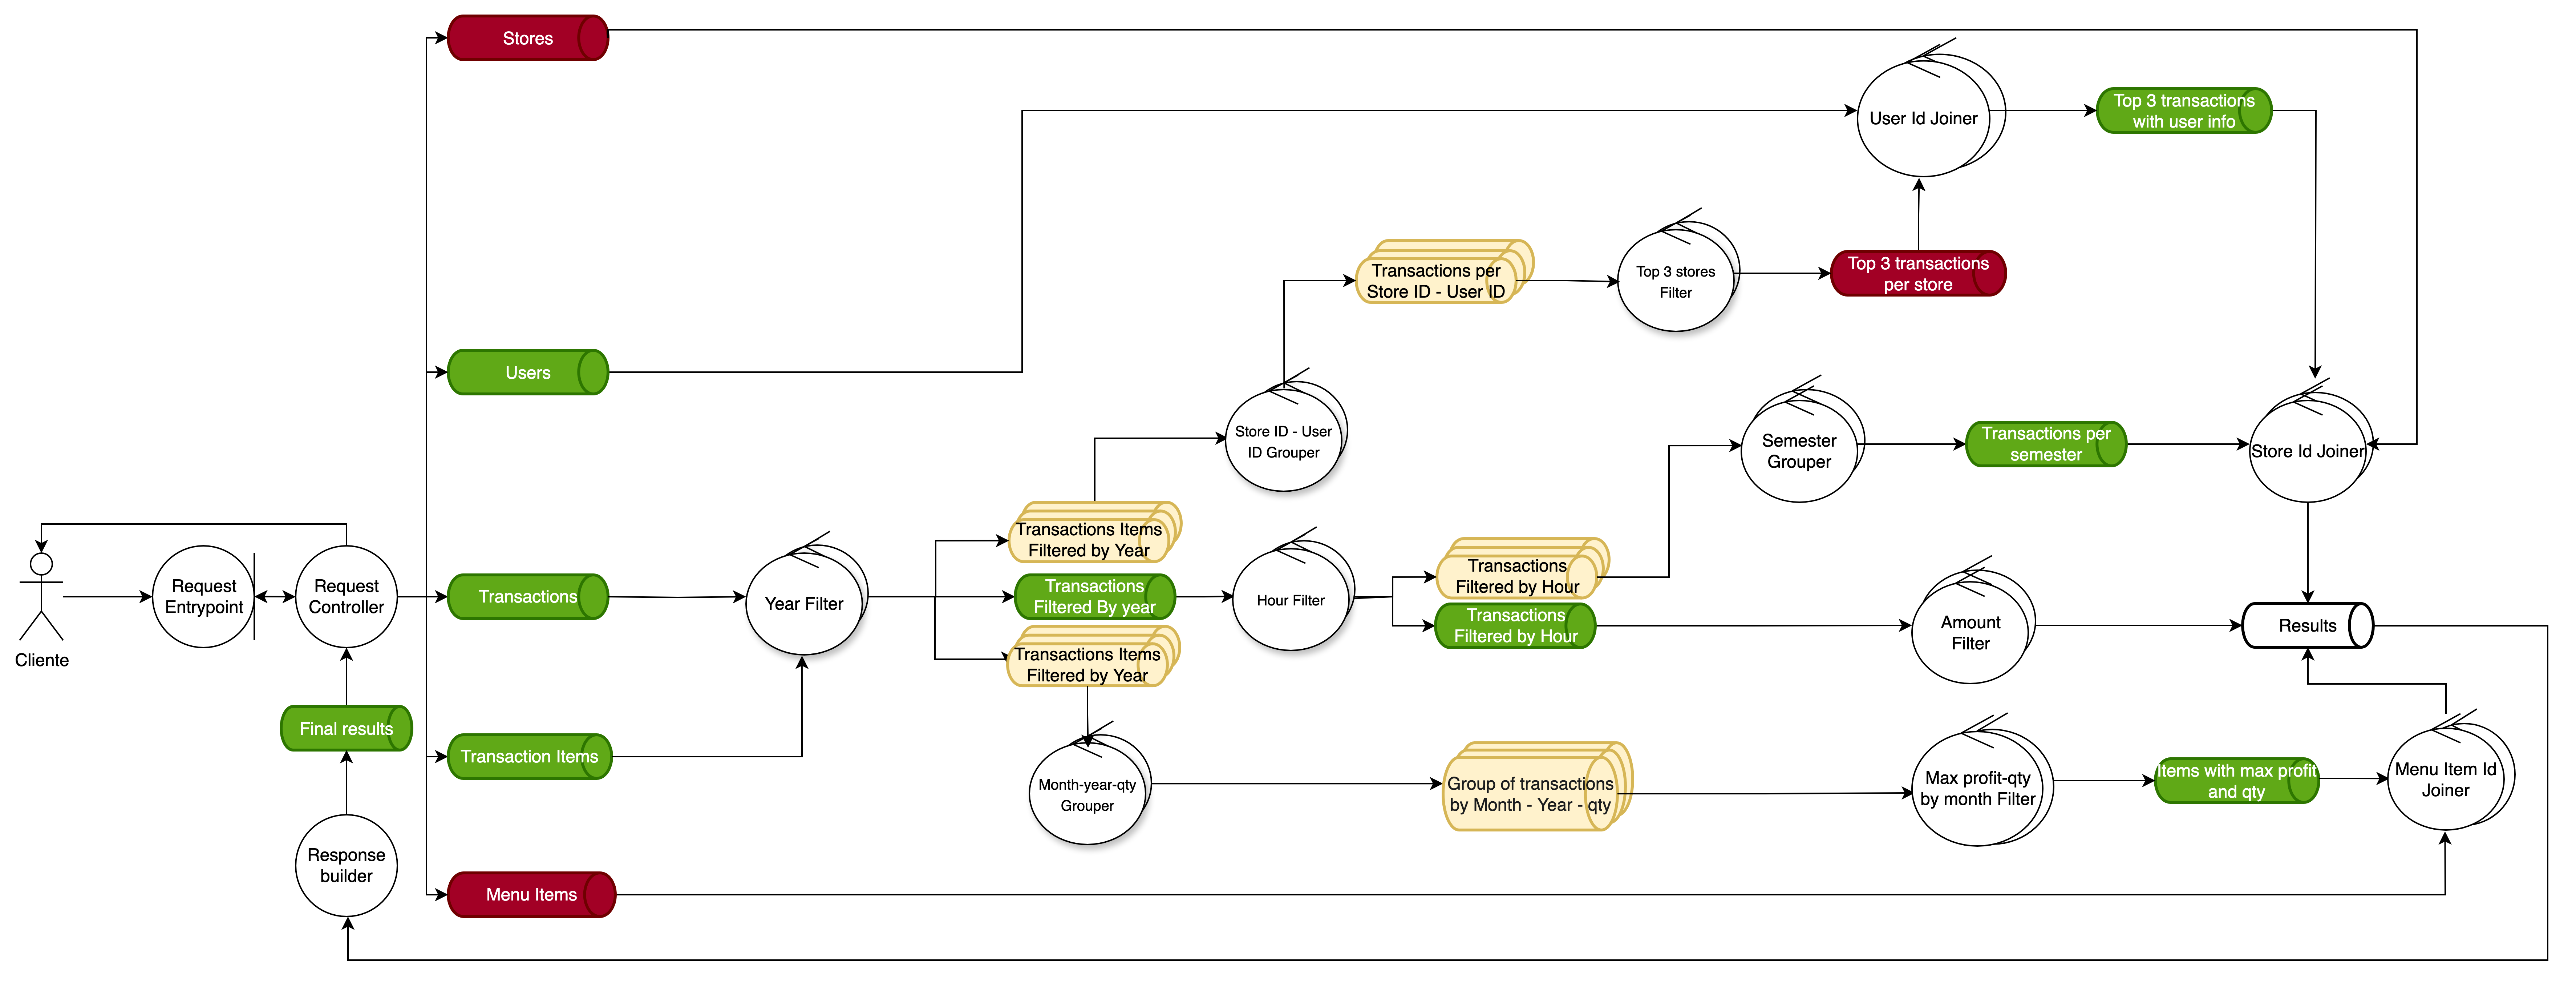
\includegraphics[width=1.4\textwidth, angle=90]{robustez.png}
\end{figure}
\paragraph{Se visualizan todos los componentes que interactuan en nuestro diseño, desde la interacción inicial del cliente, hasta la finalización del procesado de todas las consultas.}
\begin{itemize}
    \item Los trabajadores se comunican a través de la inserción y consumo de datos en diversas colas, las cuales pueden ser accedidas por multiples trabajadores en paralelo. Se distinguen 3 tipos de cola:
\begin{figure}[H]
\centering
    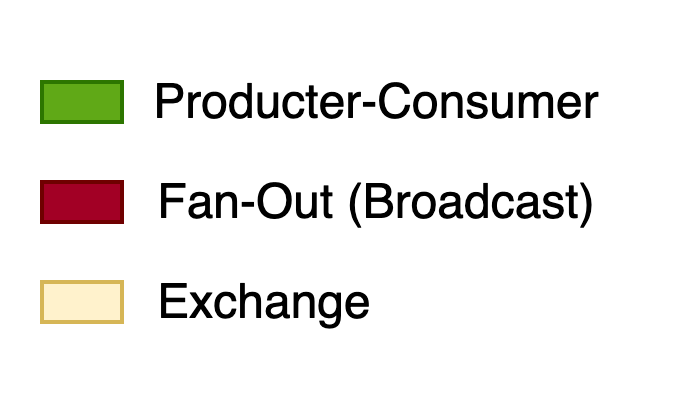
\includegraphics[width=0.45\linewidth]{colas.png}
\end{figure}

\end{itemize}
\begin{itemize}
    \item Las entidades que pueden ser escaladas a multiples unidades de computo se representan de la siguiente forma:
\begin{figure}[H]
\centering
    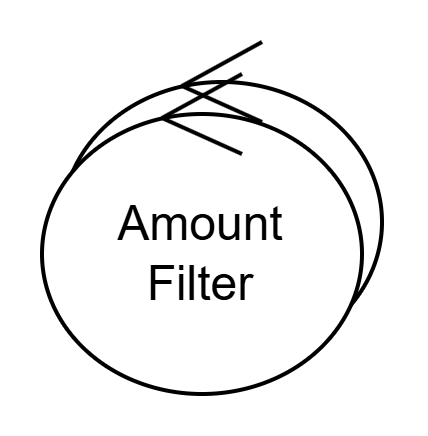
\includegraphics[width=0.15\linewidth]{multiple_computo.png}
\end{figure}
\end{itemize}

A continuación, se muestran cuatro extractos del diagrama de robustez, destacando los aspectos más relevantes de cada consulta.

\subsection*{Consulta 1}
Es la más simple. Requiere tres filtros encadenados (\textbf{Year Filter}, \textbf{Hour Filter} y \textbf{Amount Filter}).  
Cada etapa puede escalarse mediante un esquema \textbf{producer--consumer}: los workers consumen mensajes de la cola, procesan la entrada y deciden si reenviarla o descartarla.  
Los resultados de \texttt{Year Filter} y \texttt{Hour Filter} alimentan más de una cola, ya que son compartidos por otras queries.


\begin{figure}[H]
    \centering
    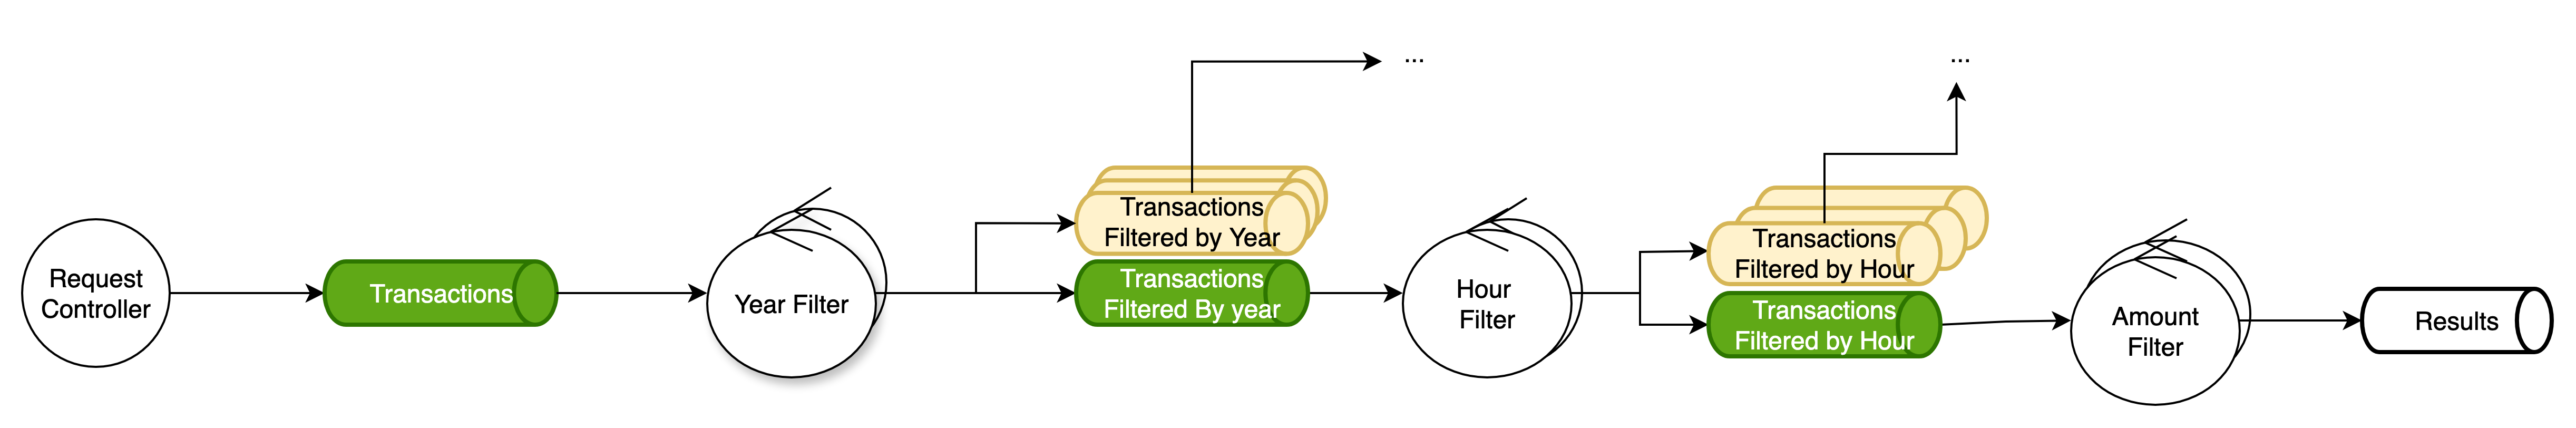
\includegraphics[width=1.0\textwidth]{consulta1.png}
    \caption{Diagrama de robustez - Consulta 1}
\end{figure}


\subsection*{Consulta 2}
Incorpora colas de tipo \textbf{exchange} y \textbf{fan-out (broadcast)}:

\begin{itemize}
    \item \textbf{Transactions Items Filtered by Year} (exchange): asegura que todas las transacciones de un mismo mes se enruten al mismo worker, asignando meses de manera balanceada entre colas. Como los pares Mes - Año conforman un total de 24 combinaciones, tendremos un total de colas y de pares procesados por worker igual a 24 / N, siendo N la cantidad de workers asignados a esta etapa.
    \item \textbf{Group of Transactions by Month--Year--Qty} (exchange): misma lógica de distribución que la anterior. Se agrupan las transacciones por año - mes - item y se realiza la suma de cantidades vendidas por producto ademas del subtotal de ganancias generadas.
    \item \textbf{Menu Items} (fan-out): los datos se difunden a todos los \texttt{Menu Item Joiner}. Estos almacenan en memoria la lista de ítems (pocos y estáticos) y luego consumen de la cola \textbf{Items with max profit and qty} (producer--consumer) para realizar los joins.
\end{itemize}

\begin{figure}[H]
    \centering
    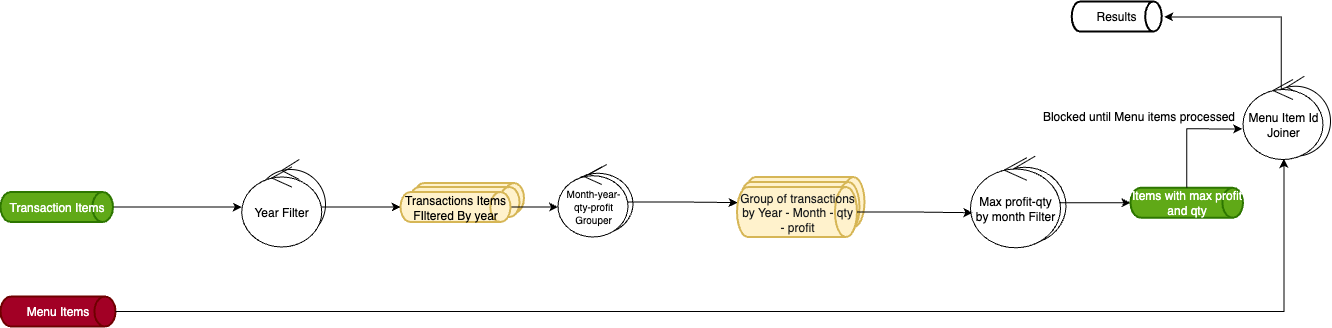
\includegraphics[width=1.0\textwidth]{consulta2.png}
    \caption{Diagrama de robustez - Consulta 2}
\end{figure}

\subsection*{Consulta 3}
Utiliza una cola de tipo \textbf{exchange}:

\begin{itemize}
    \item \textbf{Transactions Filtered by Hour}: garantiza que todas las entradas de un semestre lleguen al mismo \texttt{Semester Grouper}, que así dispone de la información completa para agregación. Como el total de semestres conforman un total de 4 posibilidades, tendremos un total de colas y de semestres procesados por worker igual a 4 / N, siendo N la cantidad de workers asignados a esta etapa.
\end{itemize}

Además, como en la Consulta 2, los \texttt{Store Id Joiner} reciben por \textbf{fan-out} todos los registros de \textbf{Stores}, los mantienen en memoria y luego consumen de la cola \textbf{Transactions per Semester}.

\begin{figure}[H]
    \centering
    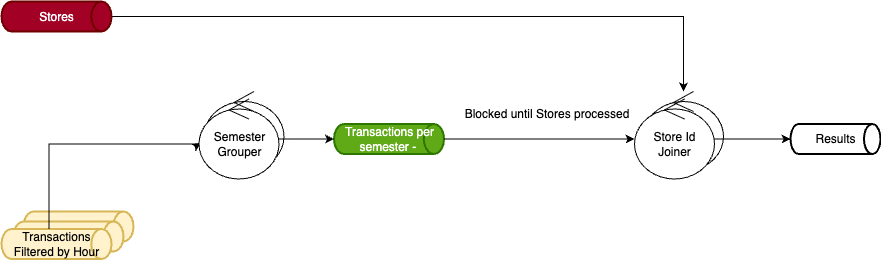
\includegraphics[width=1.0\textwidth]{consulta3.png}
    \caption{Diagrama de robustez - Consulta 3}
\end{figure}



\subsection*{Consulta 4}
Requiere dos colas de tipo \textbf{exchange}:

\begin{itemize}
    \item \textbf{Transactions Filtered by Year}: asegura que todas las transacciones de un mismo \texttt{Store ID} sean procesadas por el mismo worker. Como el total de stores conforman un total de 10 posibilidades, tendremos un total de colas y de stores procesados por worker igual a 10 / N, siendo N la cantidad de workers asignados a esta etapa.
\end{itemize}

Al igual que en las queries anteriores, las colas de tipo \textbf{fan-out} se cargan en memoria antes de iniciar el procesamiento principal.


\begin{figure}[H]
    \centering
    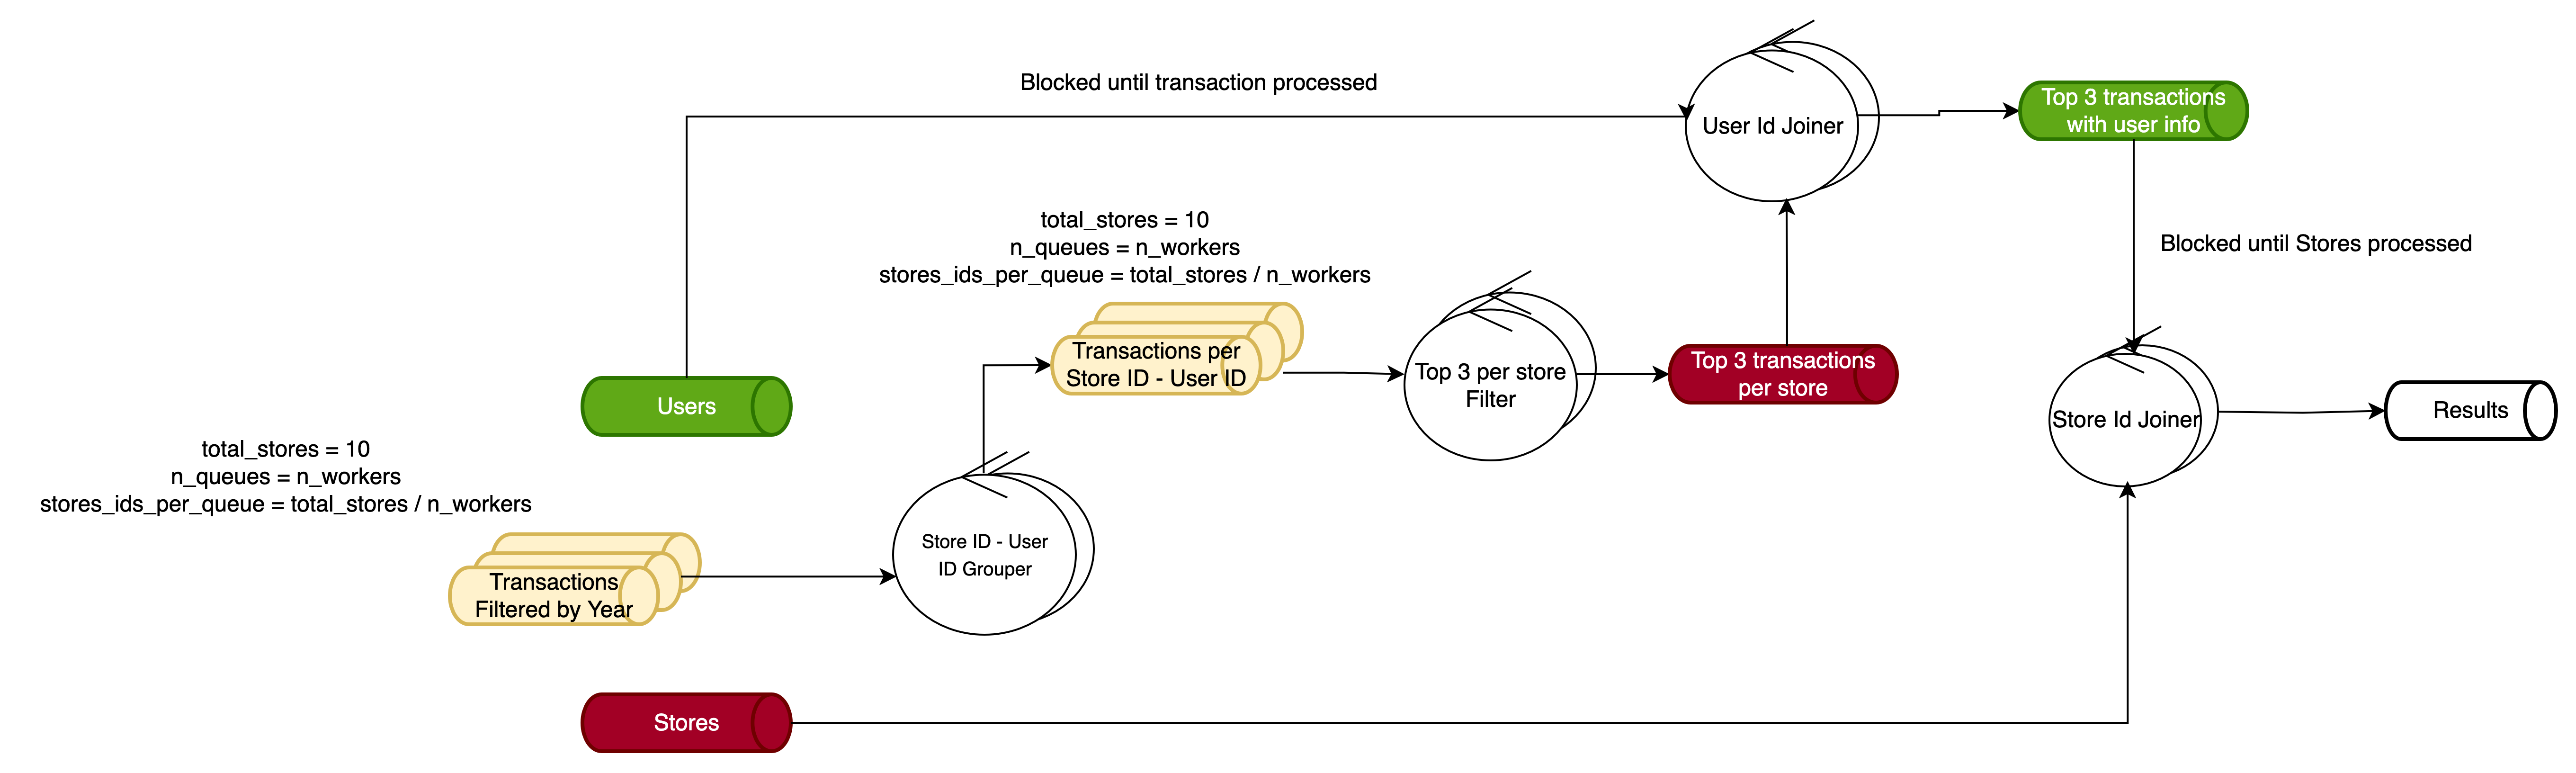
\includegraphics[width=1.0\textwidth]{consulta4.png}
    \caption{Diagrama de robustez - Consulta 4}
\end{figure}

\subsubsection{Diagrama de Despliegue}

Podemos ver como los toda comunicación interna es realizada mediante RabbitMQ (el middleware).

\begin{figure}[H]
    \centering
    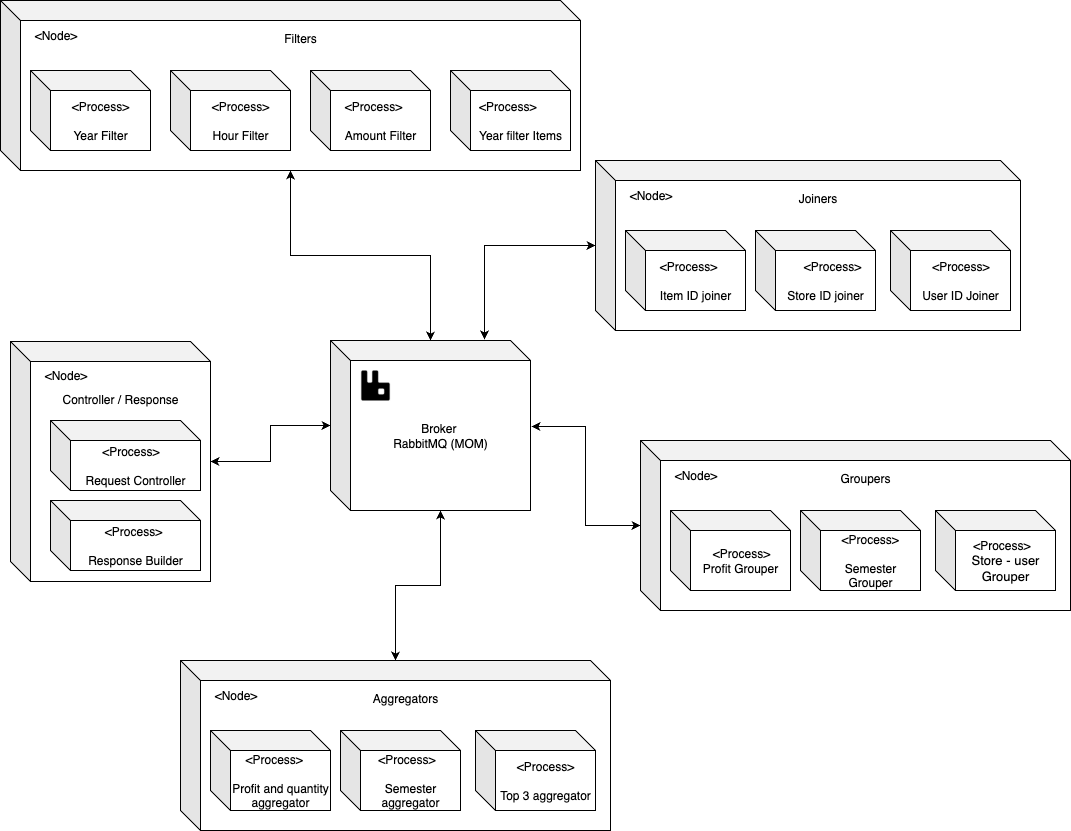
\includegraphics[width=1\linewidth]{despliegue.png}
\end{figure}


\subsection{Vista Lógica}
\subsubsection{DAG}
\begin{figure}[H]
\centering
    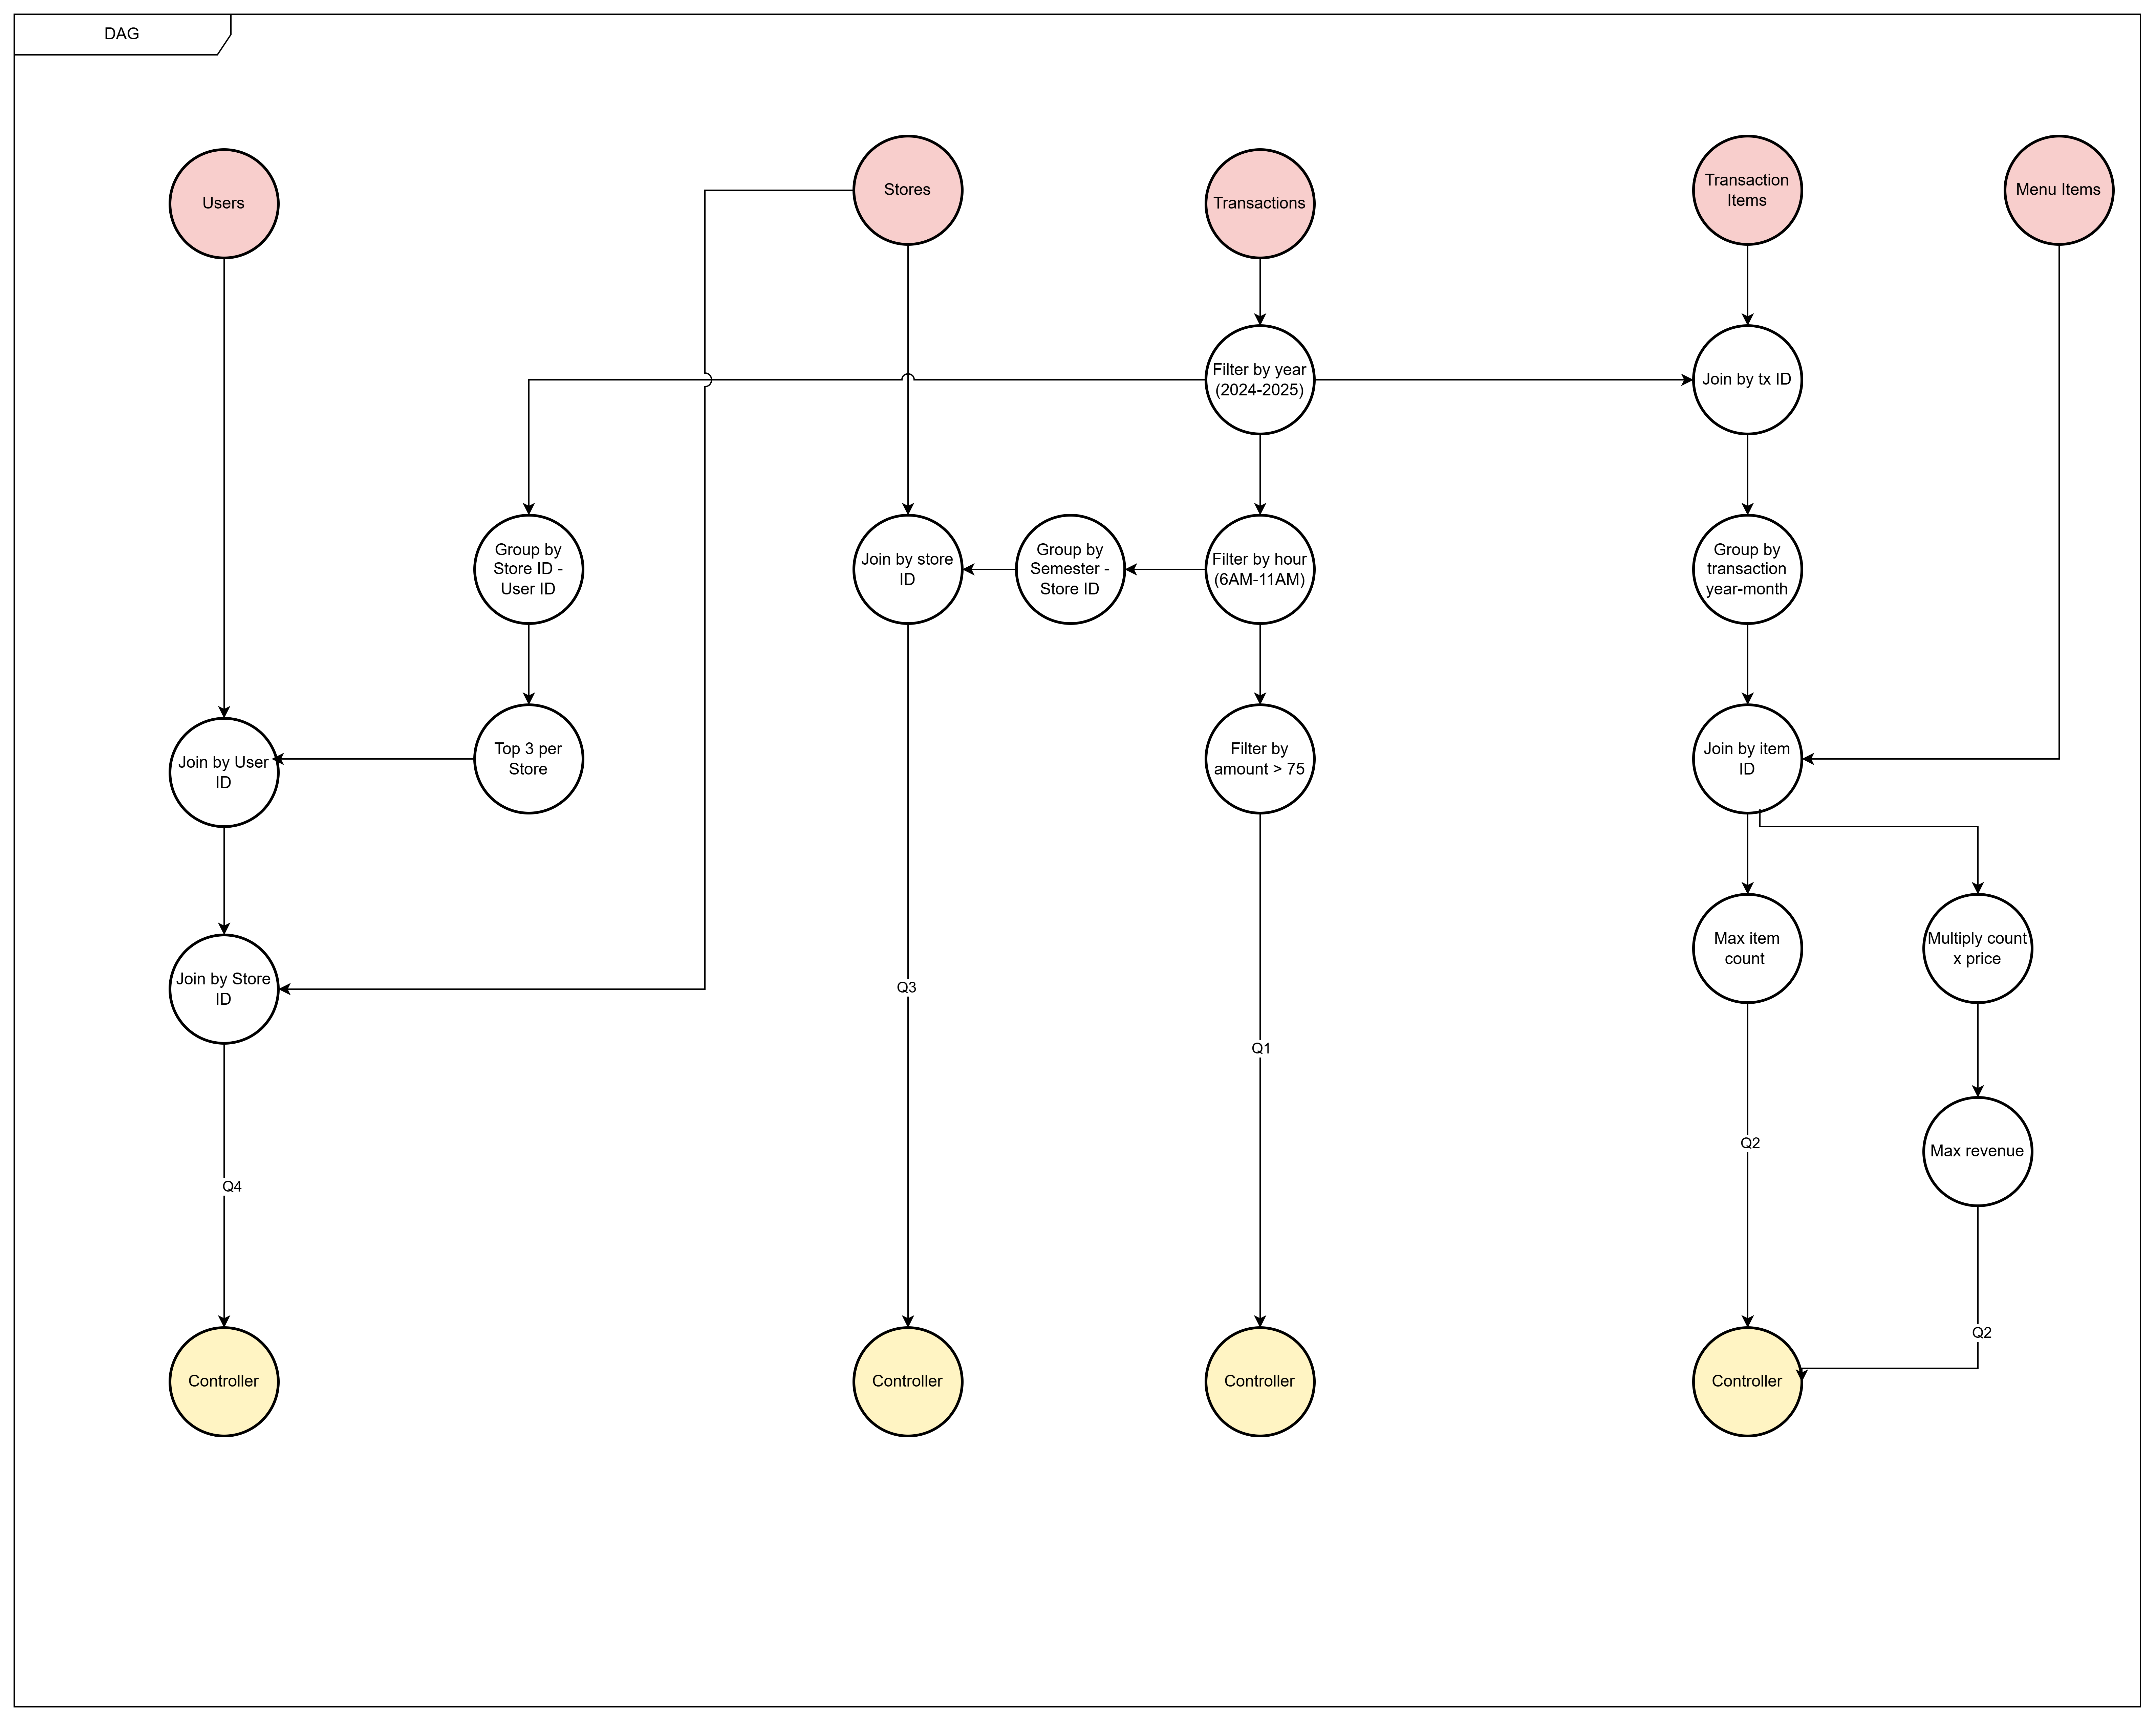
\includegraphics[width=1\linewidth]{DAG.png}
\end{figure}
Se visualiza un directed acyclic graph que muestra el flujo de datos siendo atravezado por los distintos componentes, comenzando de arriba hacia abajo. Los trabajadores (workers) se dividen en agrupadores (groupers), acumuladores (joiners) y filtradores (filters). Las fuentes de información inicial, y donde se almacena finalmente lo procesado son a nivel de implementación colas.

\subsection{Vista de Desarrollo}
Aquí podemos visualizar como esta planeada la arquitectura del sistema desde la perspectiva del código. Se divide el sistema en distintos modulos para Cliente, Worker, Request Controller y Middleware.

\subsubsection{Diagrama de Paquetes}
Se muestran los distintos modulos a implementar:
\begin{figure}[H]
    \centering
    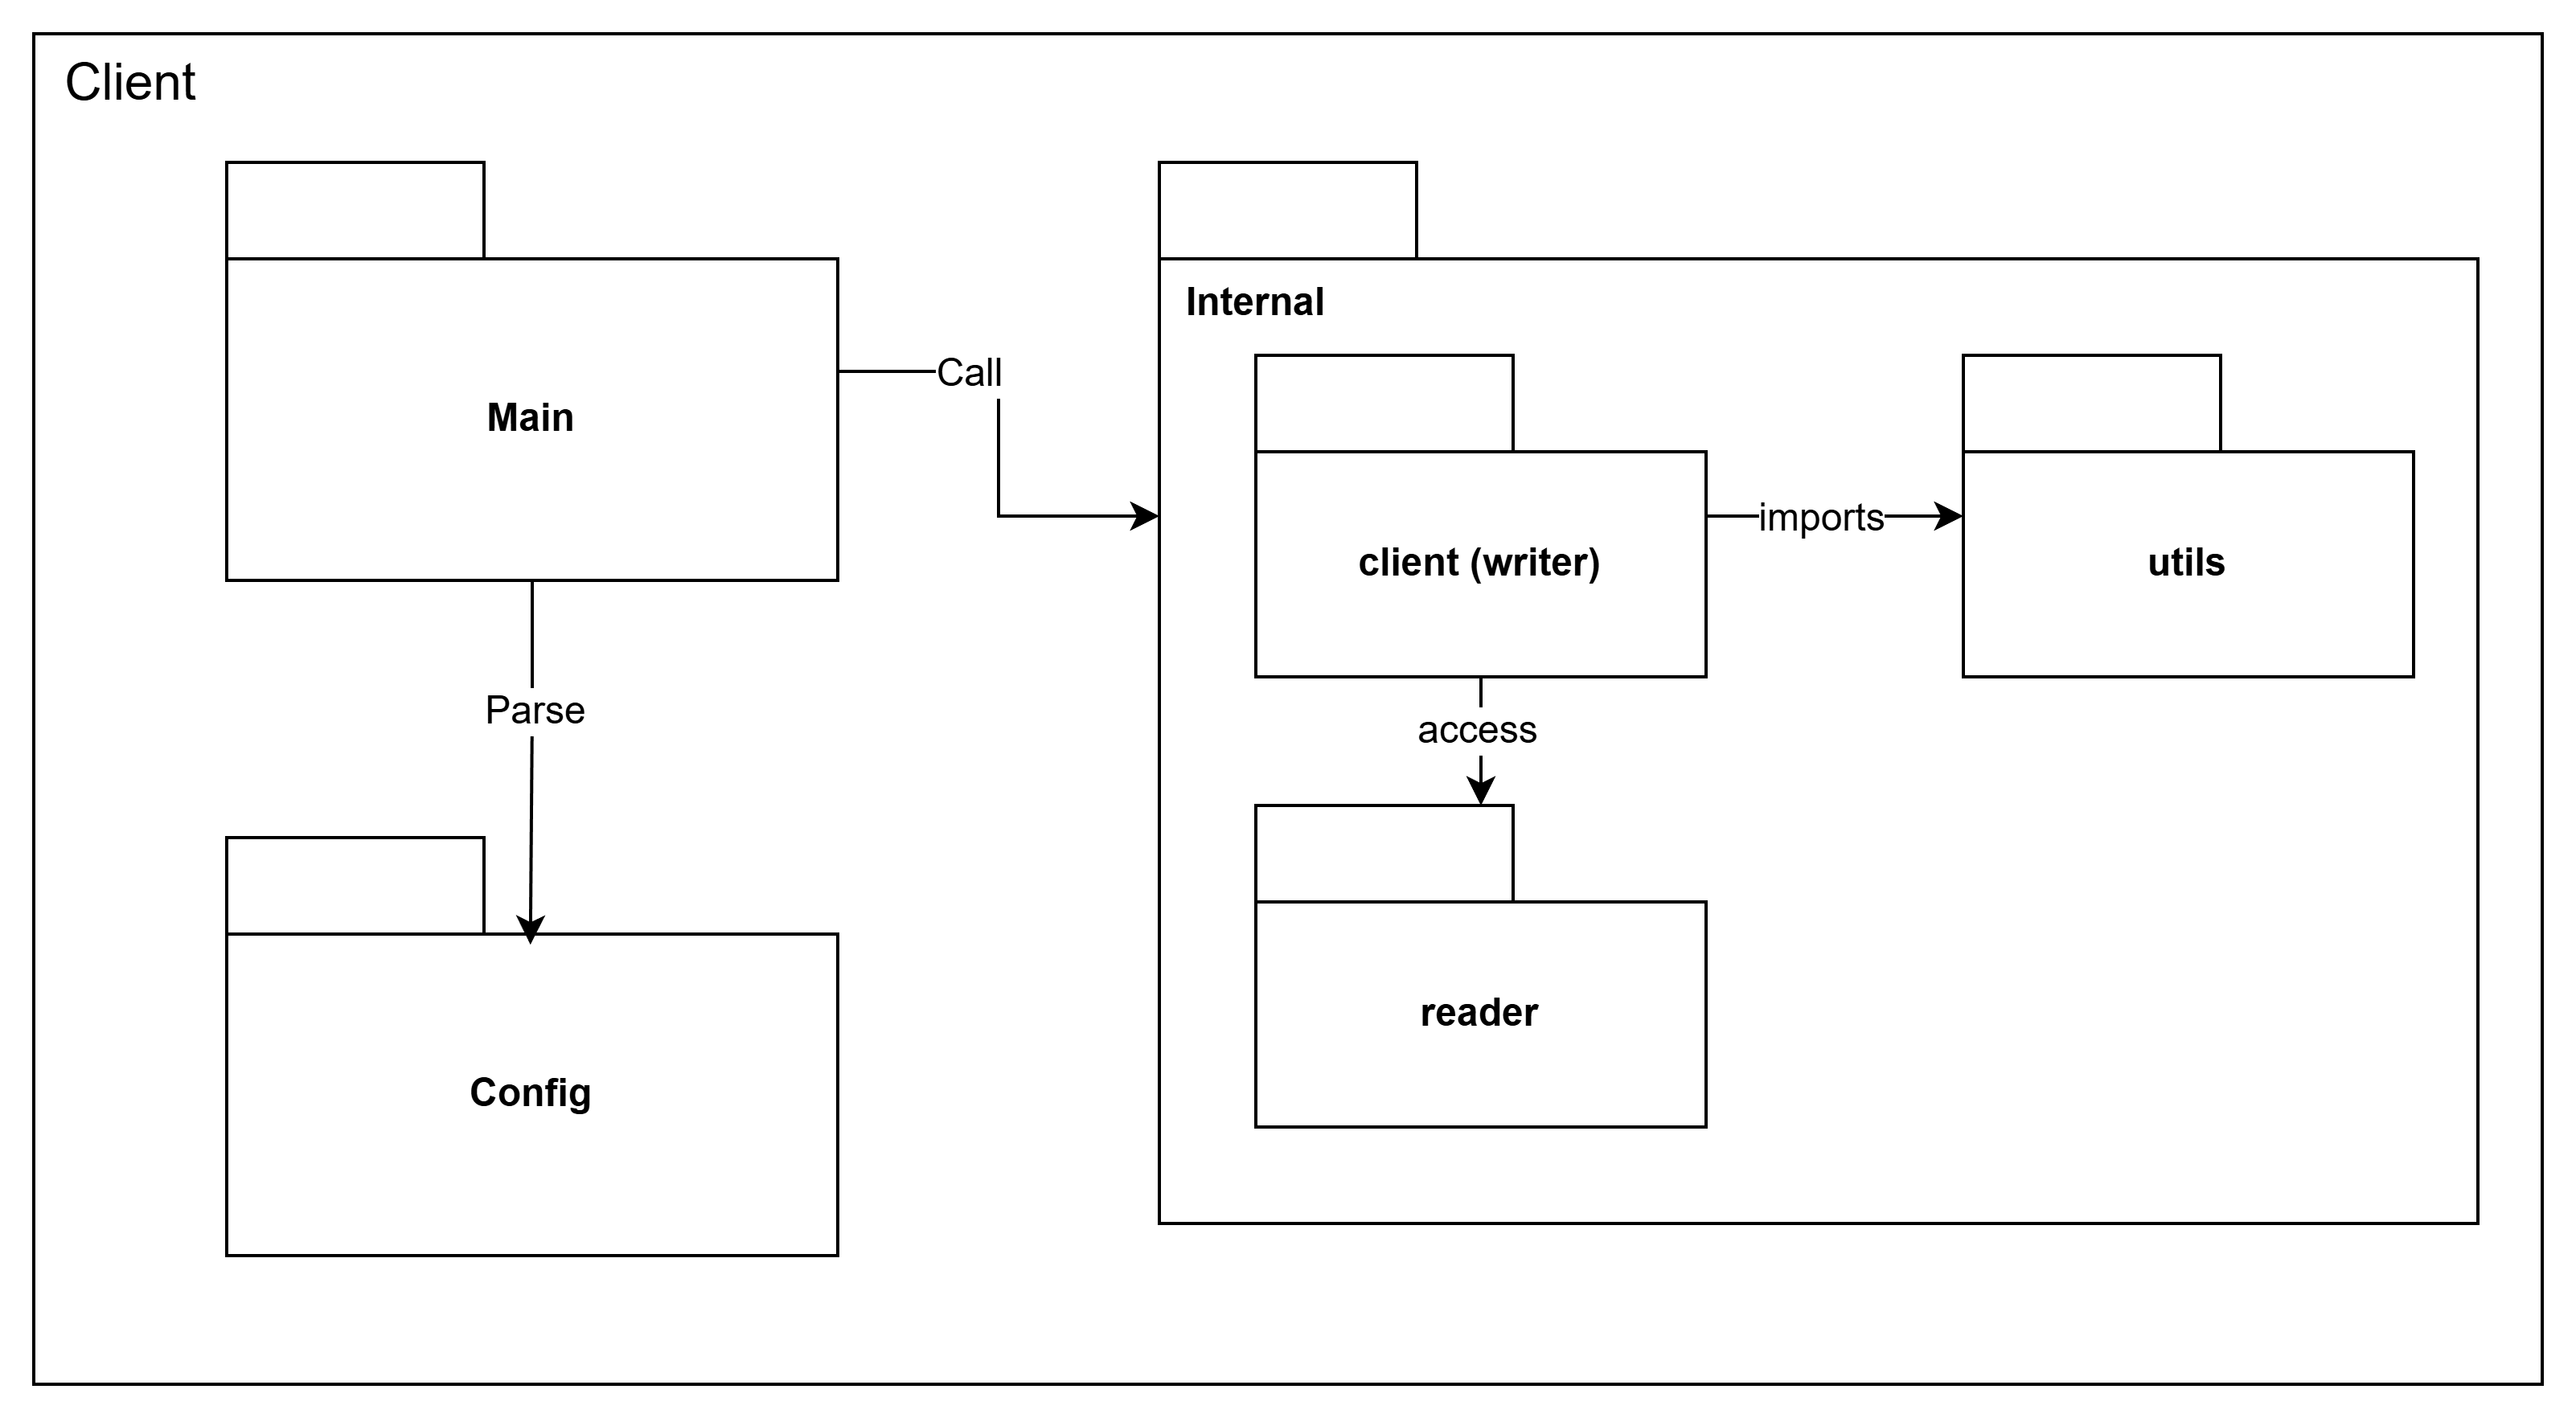
\includegraphics[width=1\linewidth]{cliente.png}
    \caption{El cliente tiene la responsabilidad de comunicarse con el Request controller, siguiendo los parametros especificados en su configuración.}
\end{figure}
\begin{figure}[H]
    \centering
    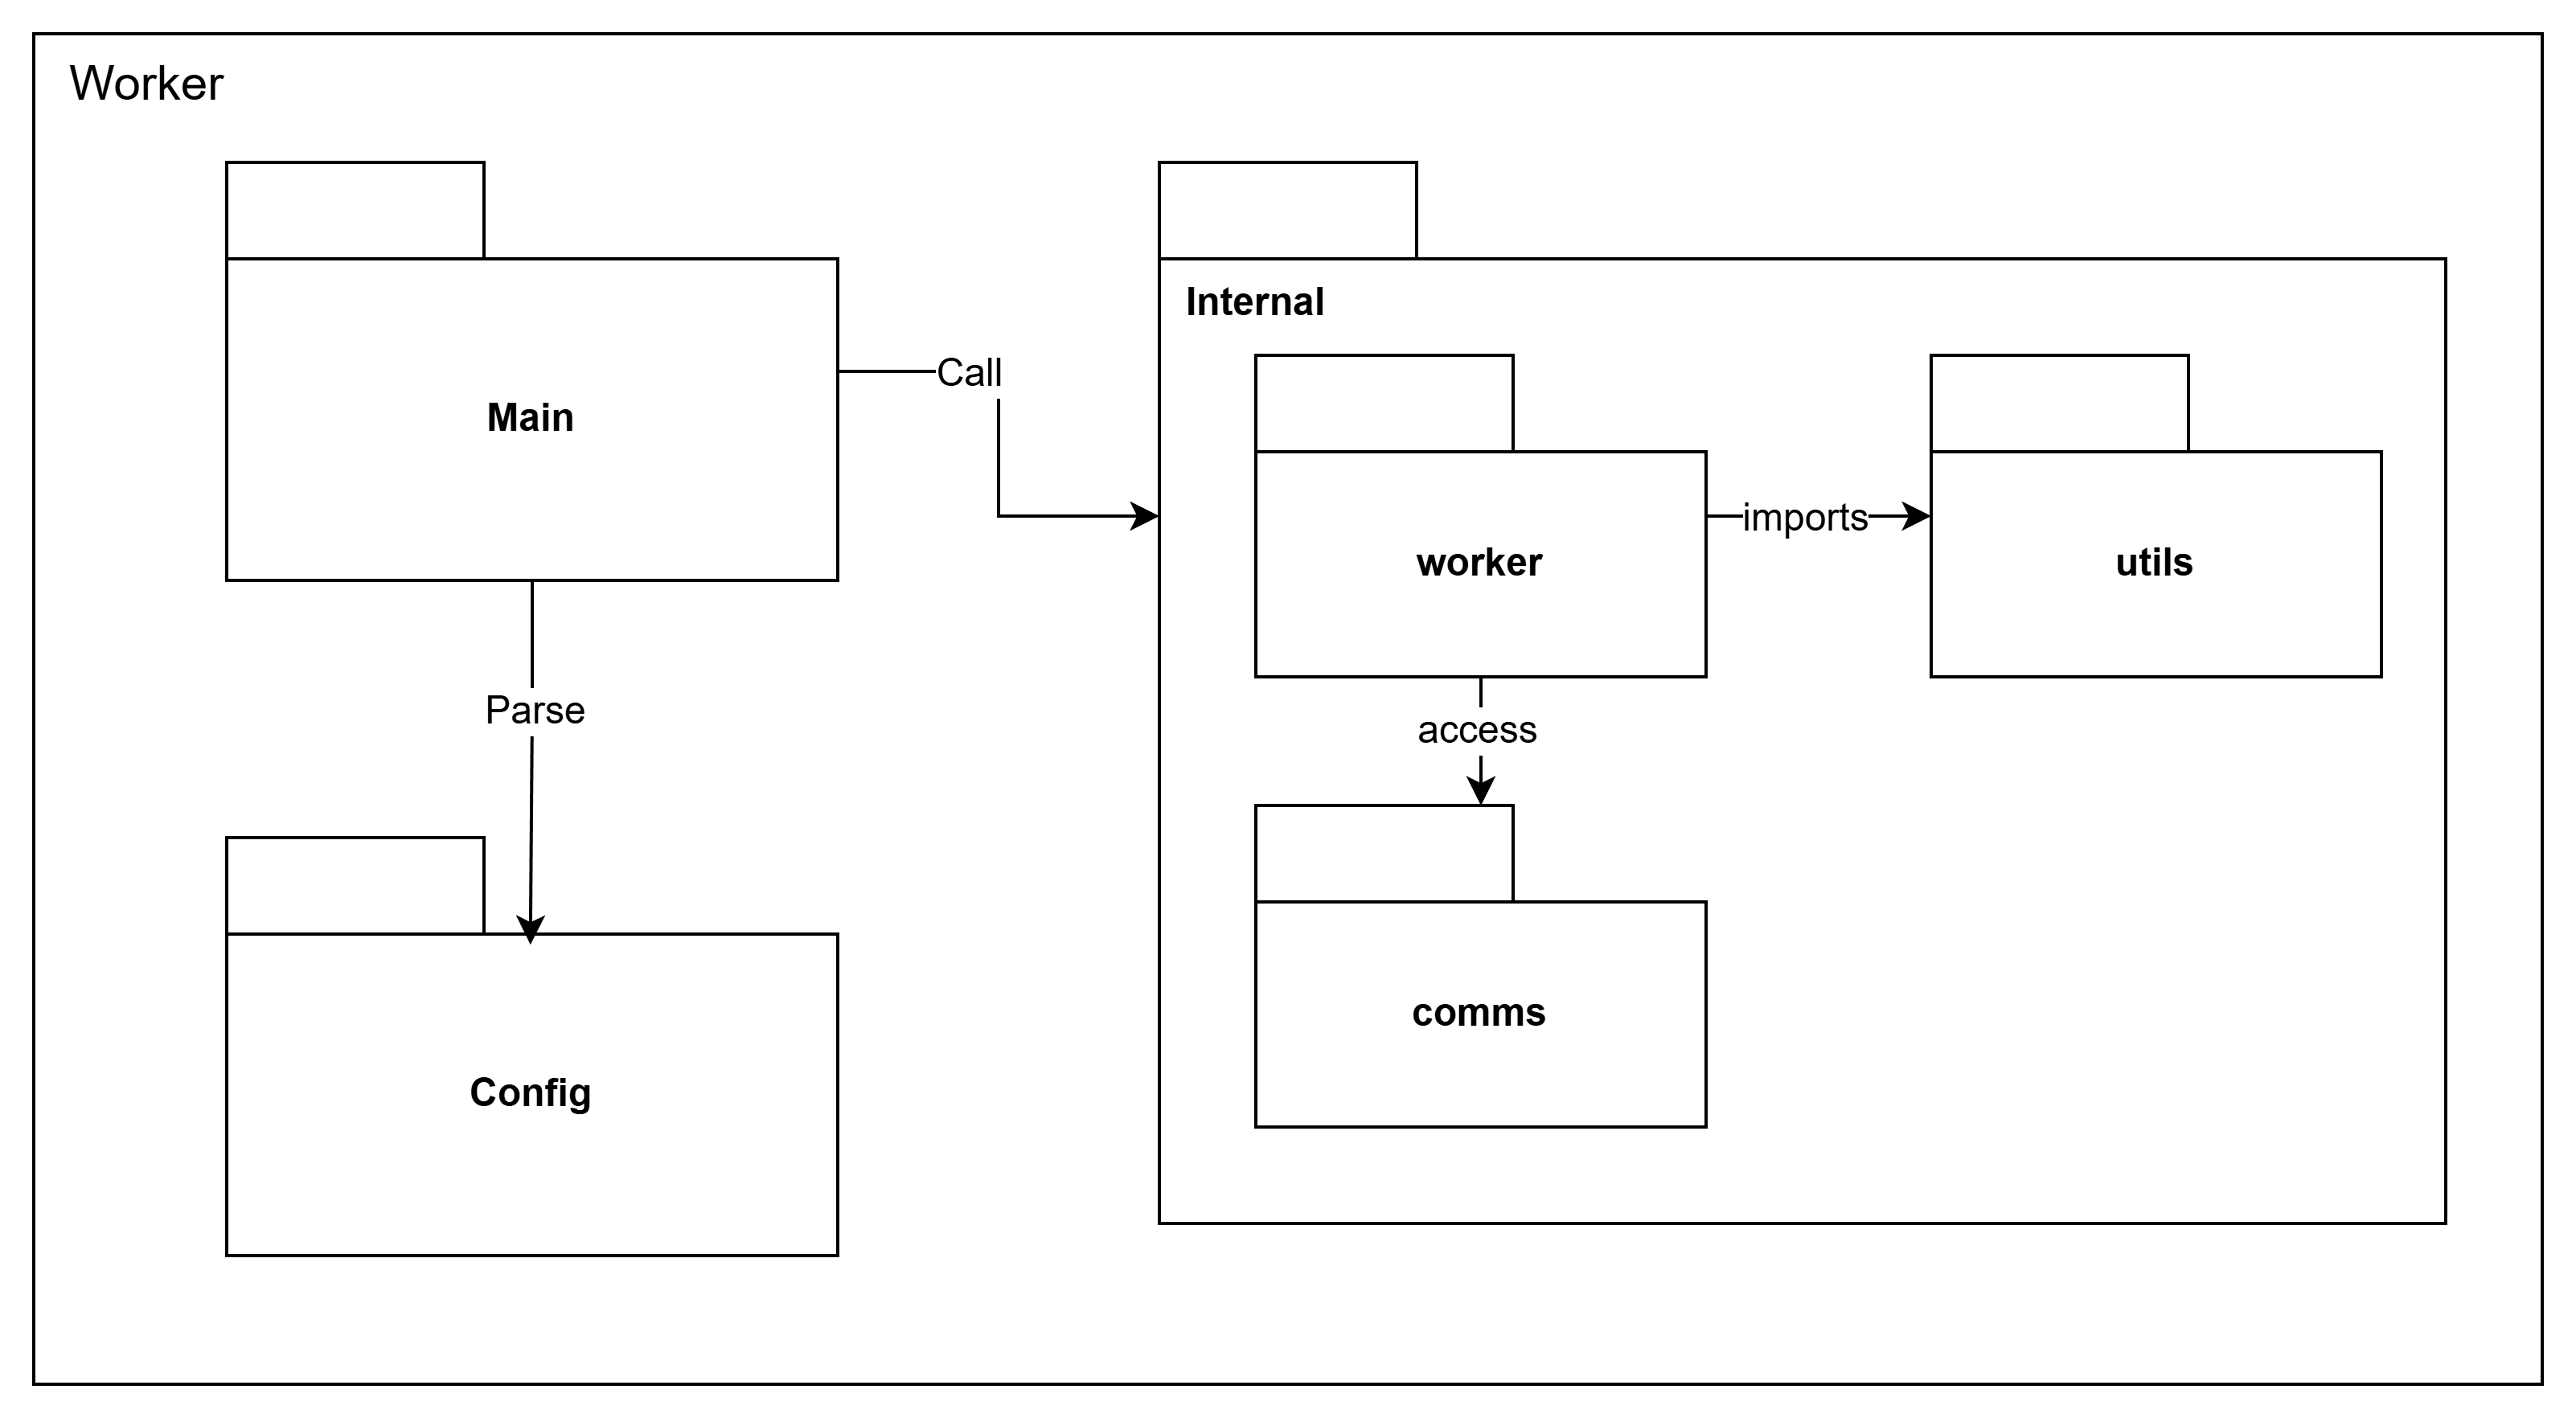
\includegraphics[width=1\linewidth]{worker.png}
    \caption{Los workers tienen la tarea de filtrar, acumular o agrupar los diversos tipos de datos que lean de las colas a las que estes subscriptos.}
\end{figure}

\begin{figure}[H]
    \centering
    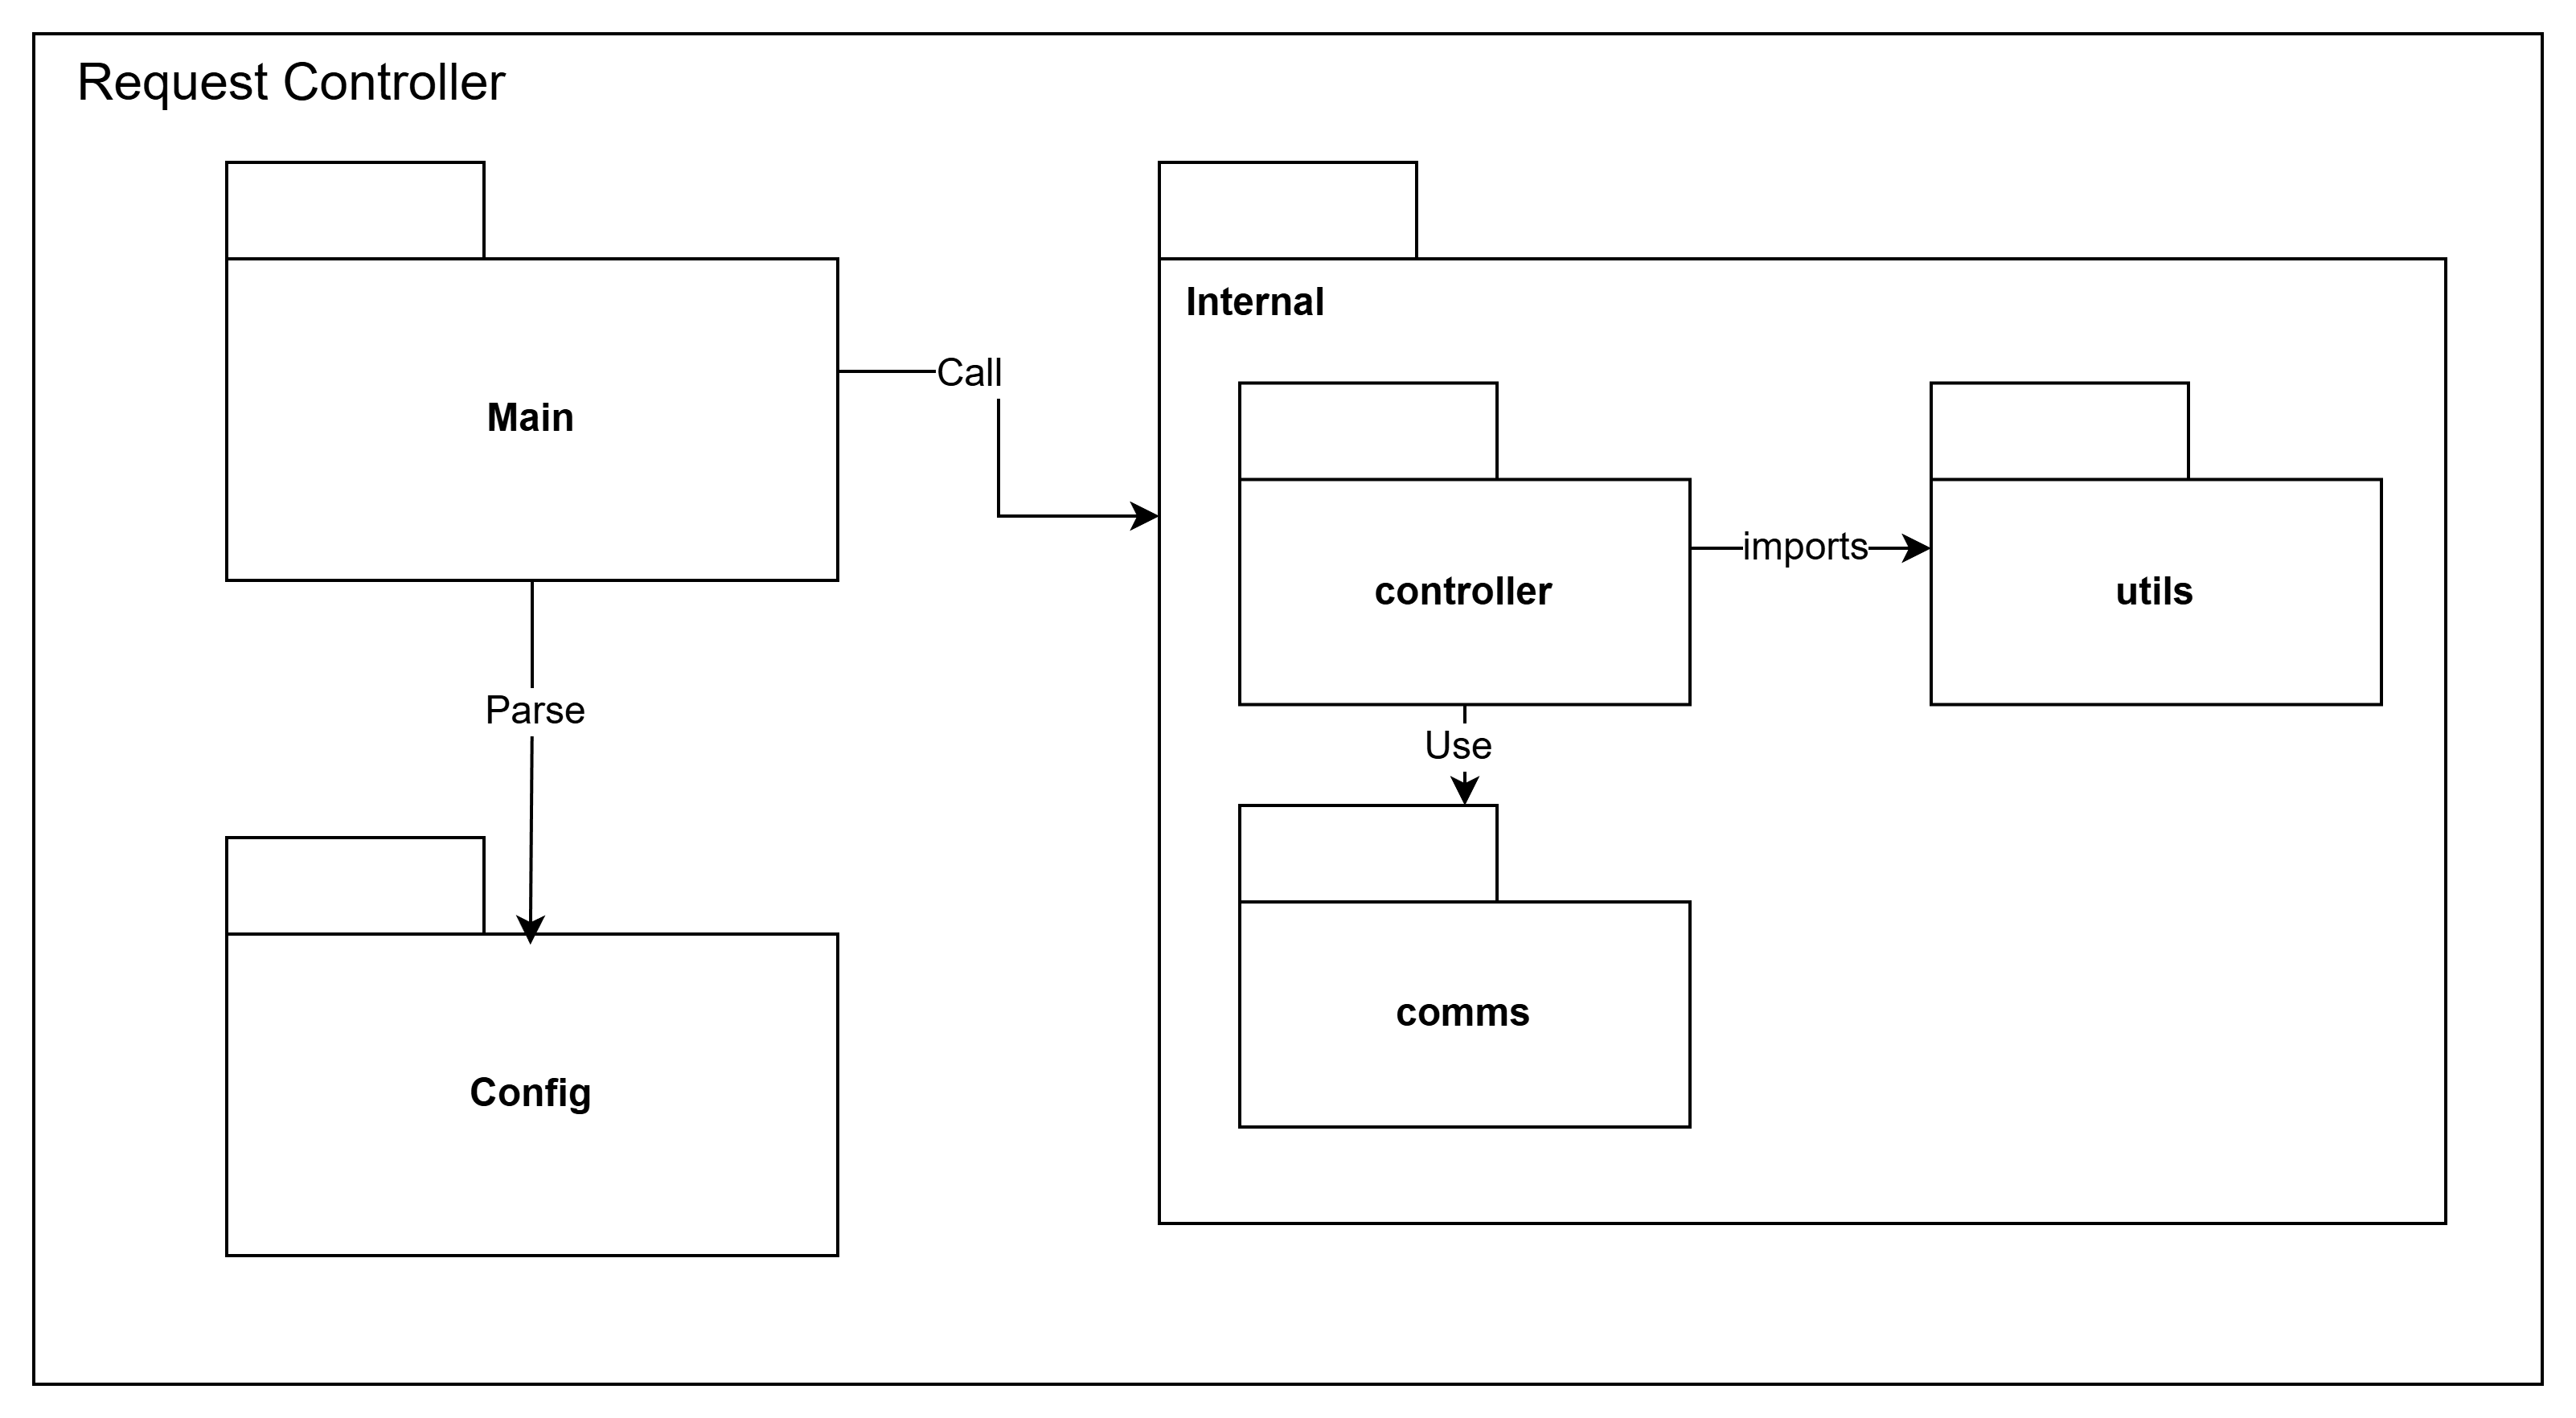
\includegraphics[width=1\linewidth]{request_controller.png}
    \caption{La tarea del request controller es interpretar los mensajes del cliente, para poder derivarlos a las diferentes colas de RabbitMQ.}
\end{figure}

\begin{figure}[H]
    \centering
    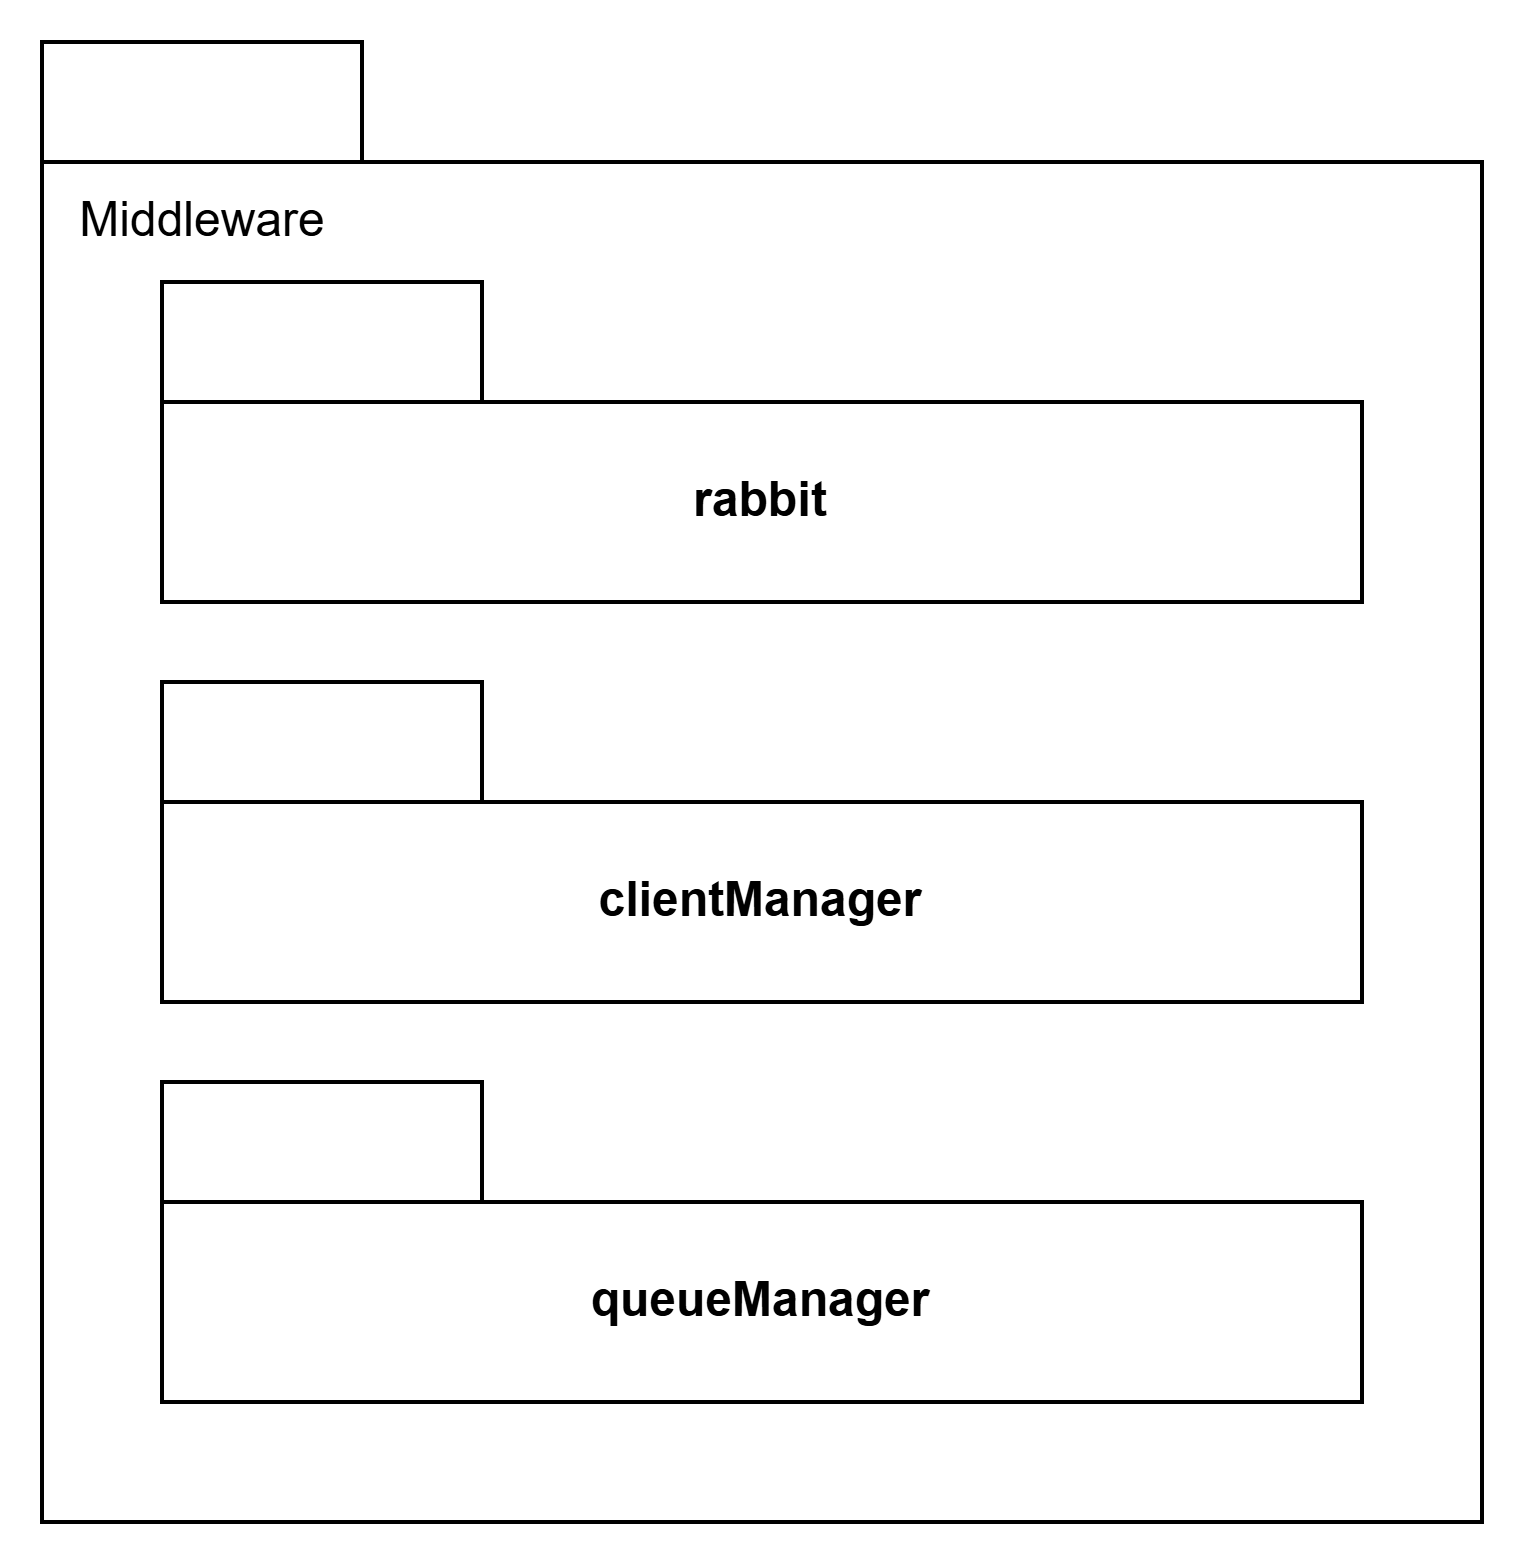
\includegraphics[width=0.45\linewidth]{middleware.png}
    \caption{El Middleware tiene un manejo de cola y cliente, asi como también las librerias necesarias para el interfazado con RabbitMQ}
\end{figure}
\begin{figure}
    \centering
    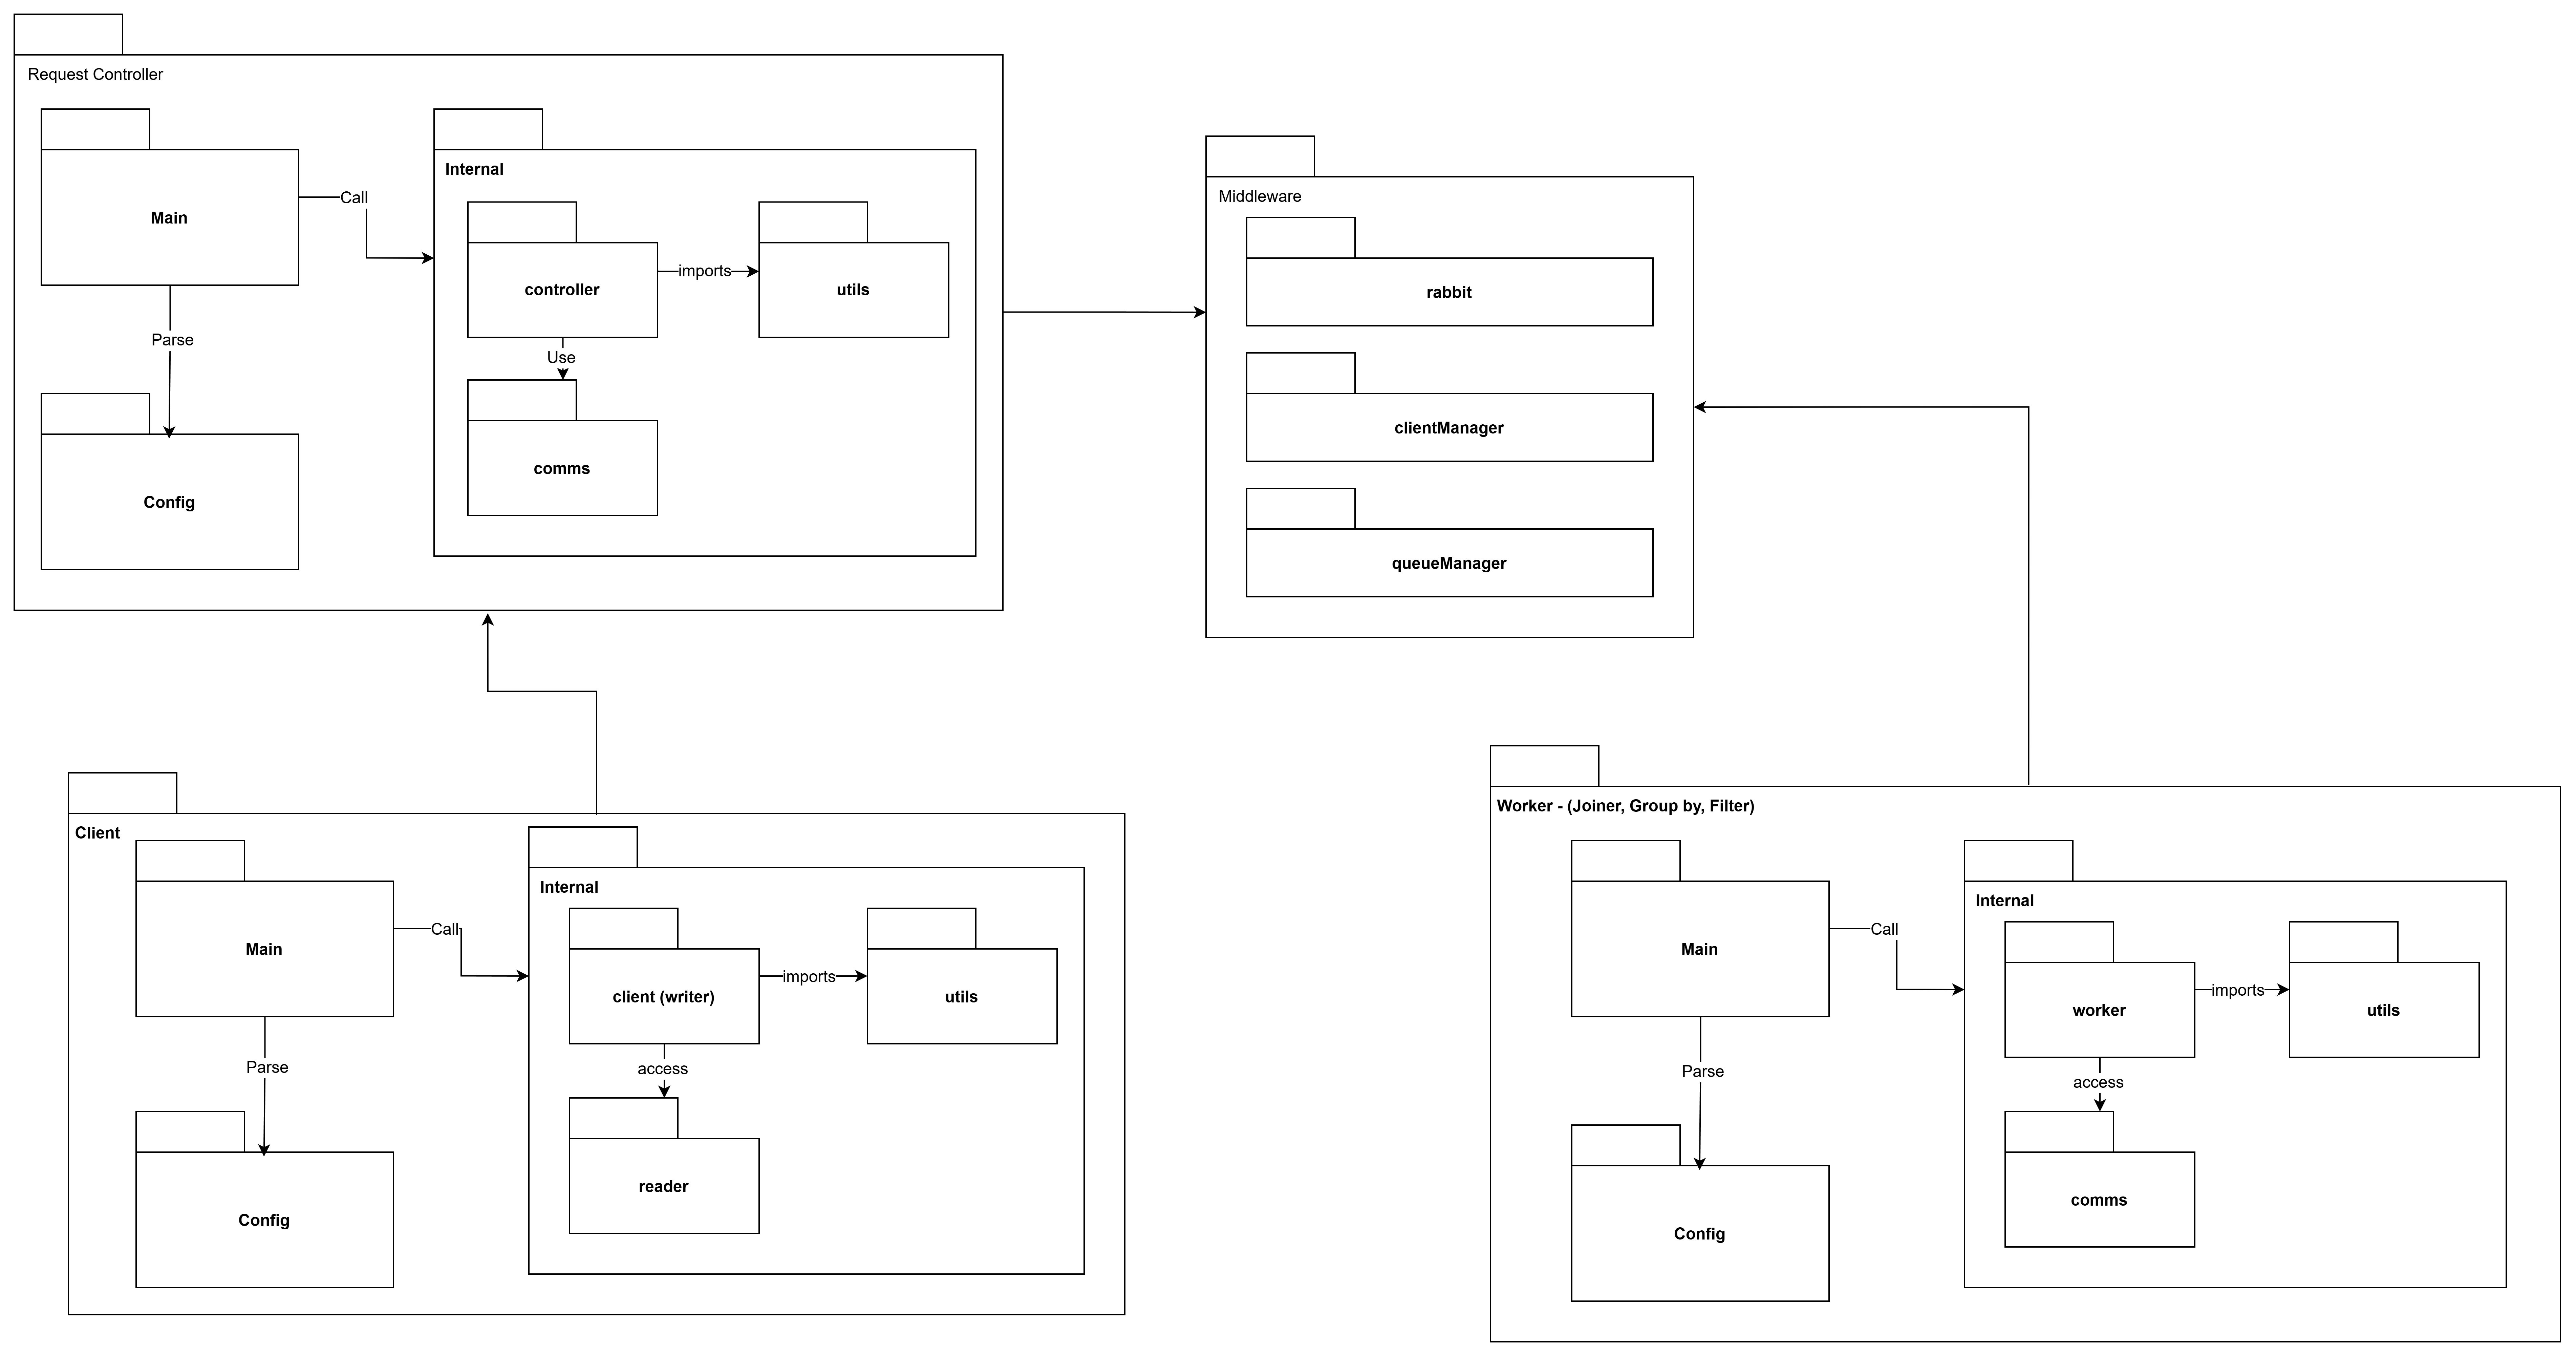
\includegraphics[width=1.4\textwidth, angle=90]{general.png}
    \caption{Vista general de los paquetes, incluyendo la comunicación entre estos.}
\end{figure}

\subsection{Vista de Procesos}

\paragraph{Se representa la interacción entre los componentes del sistema, su forma de comunicación de principio a fin. Es posible visualizar la concurrencia del sistema, asi como también la escalabilidad y distribuición de tareas.}

\subsubsection{Diagrama de Actividad}
\begin{figure}[H]
    \centering
    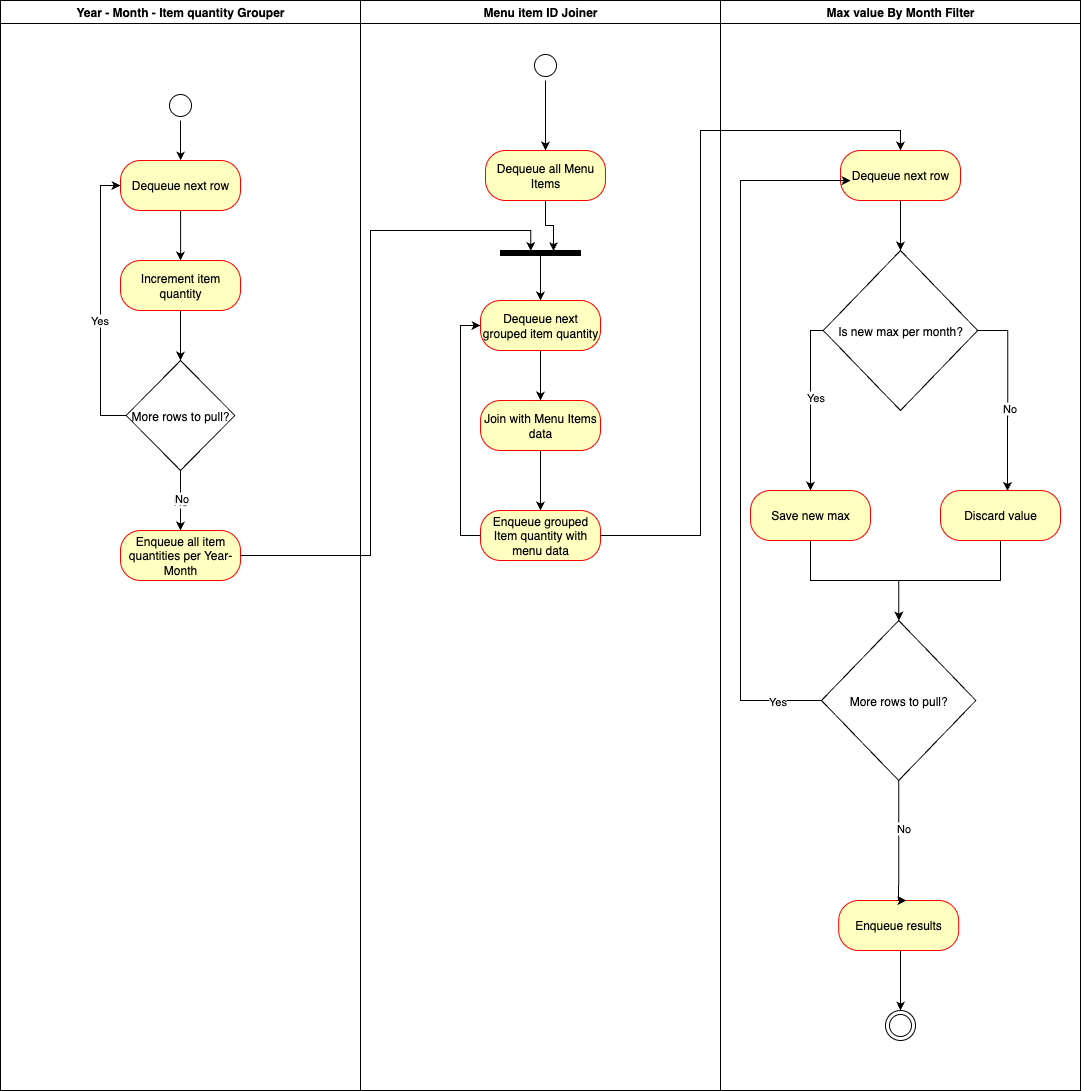
\includegraphics[width=1\linewidth]{actividad.png}
\end{figure}
\paragraph{Se muestra el parcialmente el proceso de obtener los productos más vendidos y que más ganancias han generado, para cada mes, en este caso se representa solamente la parte de mayor complejidad* de obtención, la de mayor valor y no solo mayor cantidad de ventas.}

\paragraph{*Se considera más complejo debido a que los pasos necesarios para obtener este dato es superior a la de calcular el producto más vendido en cantidad.}

\subsubsection{Diagrama de Secuencia}

\begin{figure}[H]
    \centering
    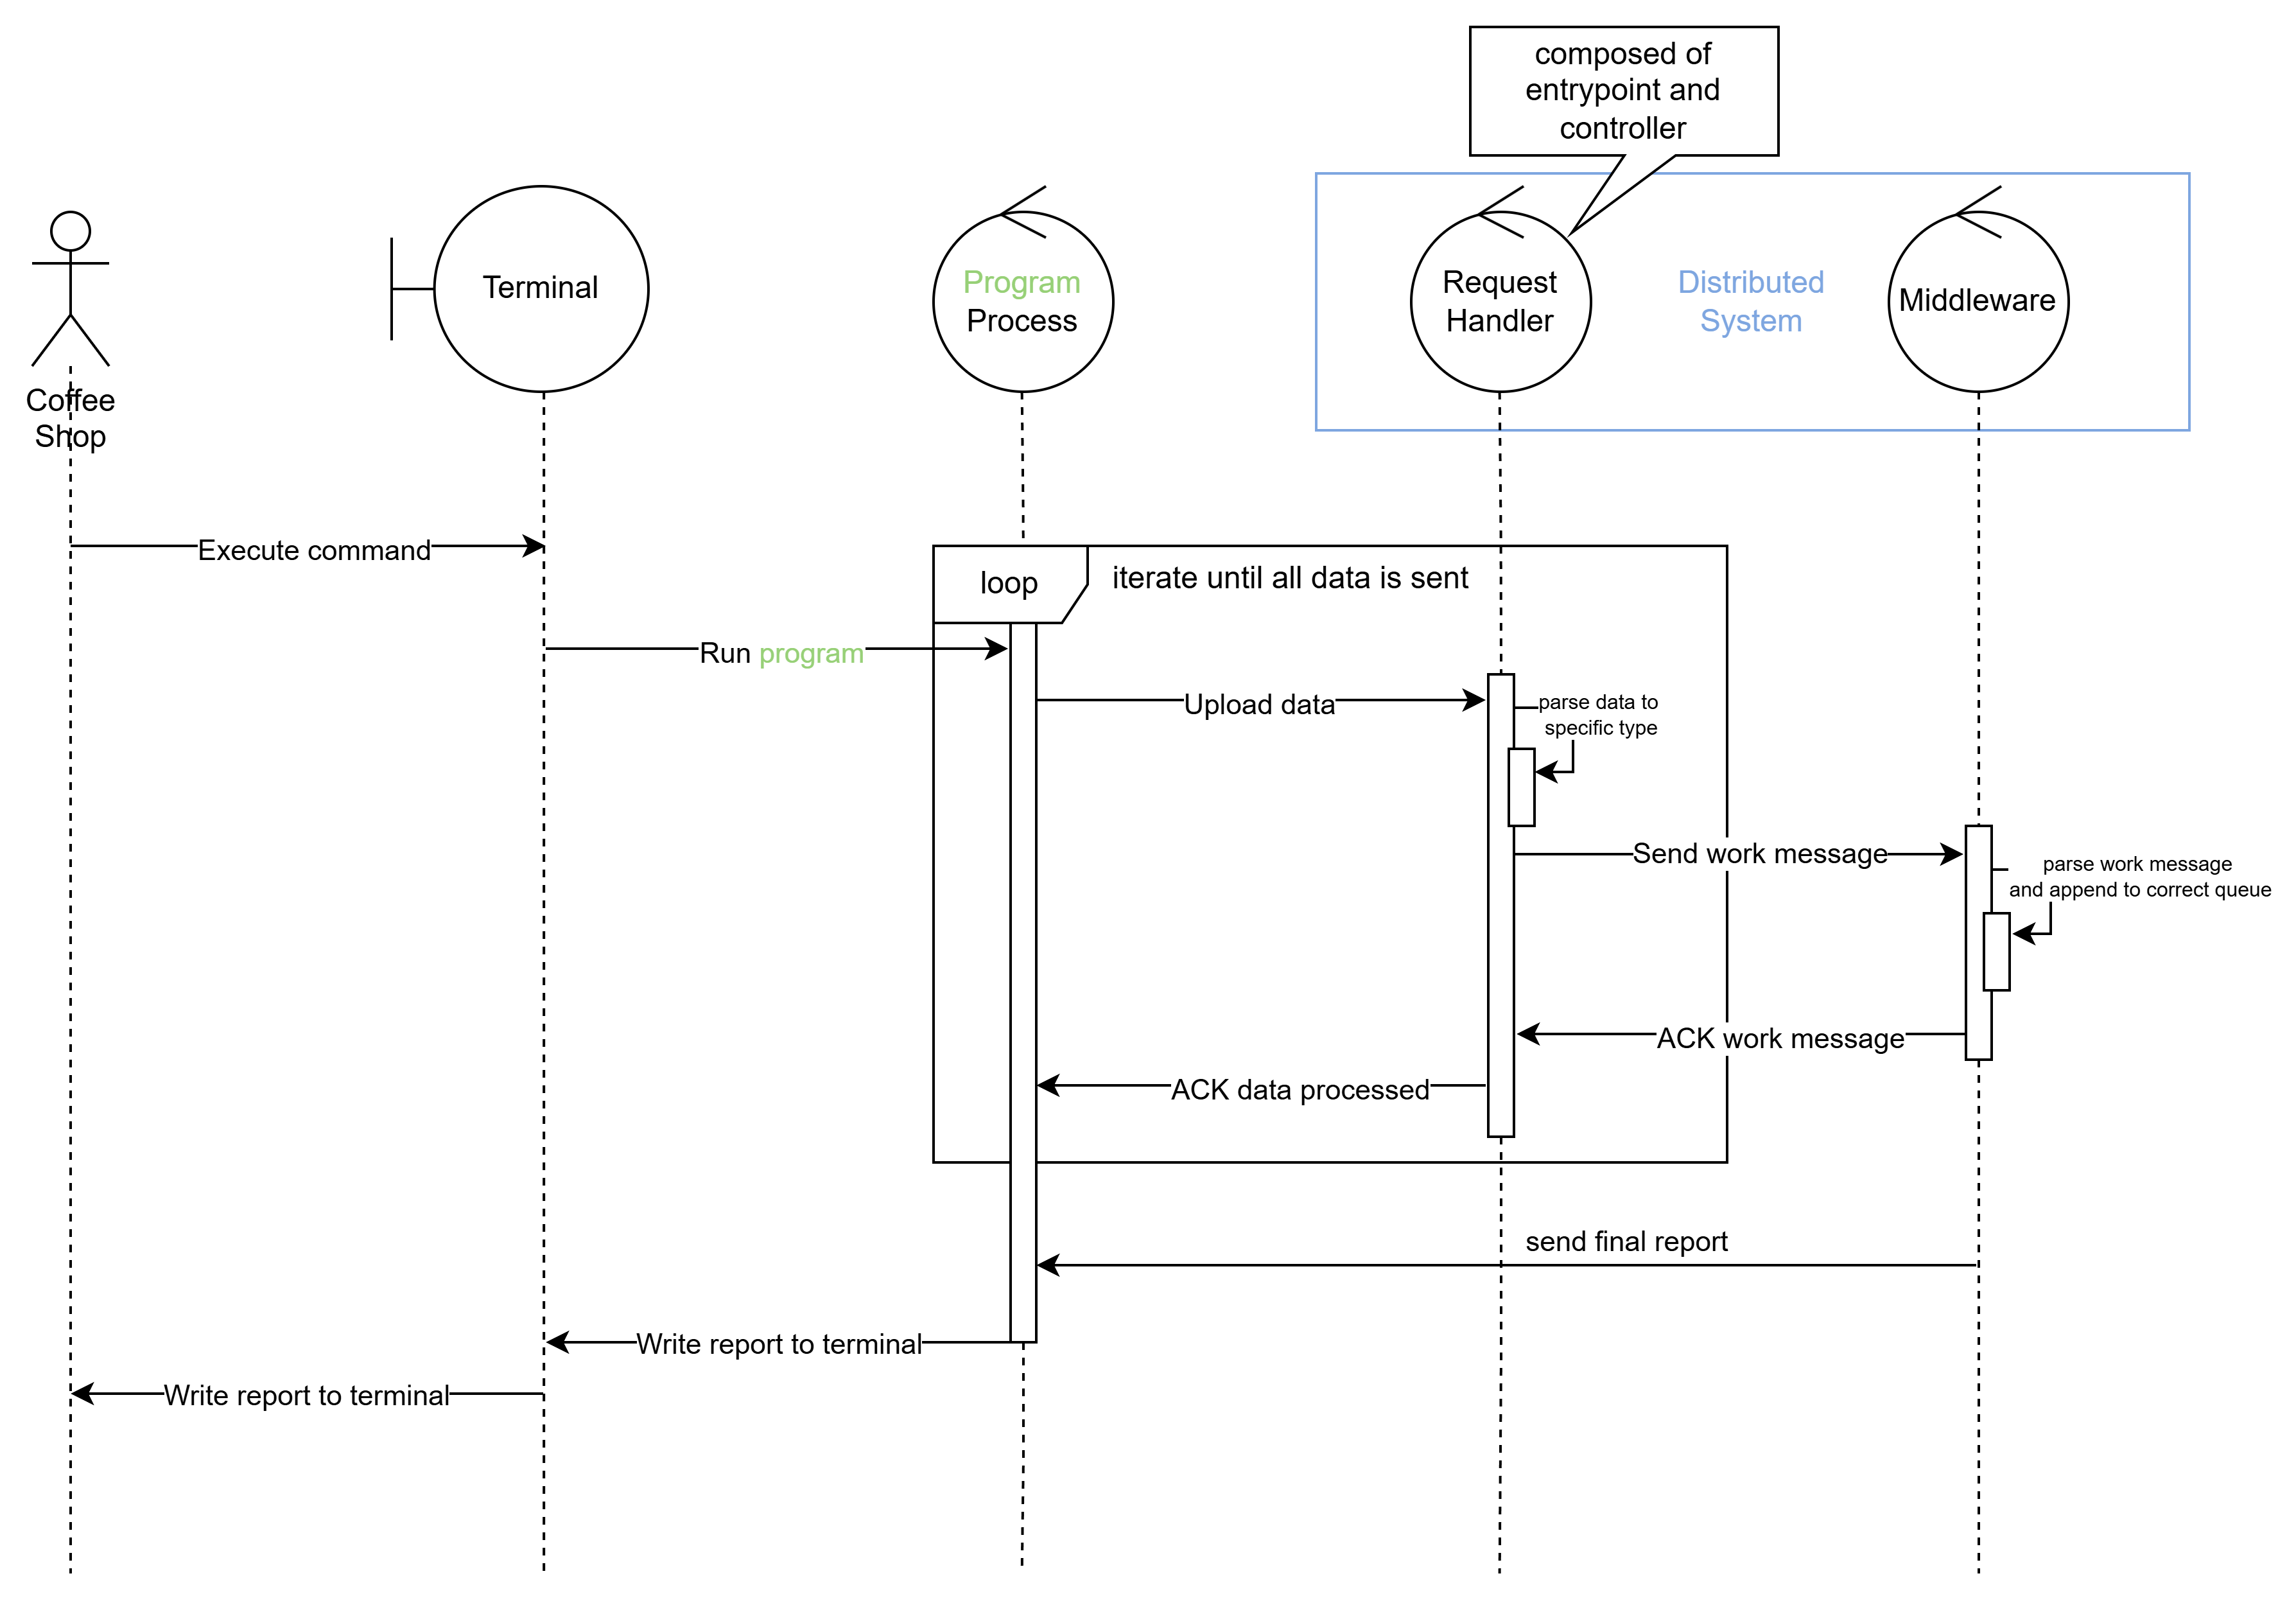
\includegraphics[width=1\linewidth]{secuencia.png}
\end{figure}
\paragraph{Podemos ver como el cliente desde la terminal inicializa el programa, el cual establece conexión con el sistema mediante el Request Handler. La comunicación entre ellos consistira en enviar todos los datos necesarios en bucle, cada mensaje transmitido por el cliente incluye un header informando el tipo de archivo transmitido, el tamaño del payload, y un bit que indica si hay datos pendientes por transmitir posteriores a ese mensaje. Una vez que ya no haya nada más que enviar, el Middleware le enviará el programa el resultado final, el cual sera mostrado por terminal al usuario.}
\end{document}
